
\documentclass[a4paper,compress]{beamer}
%\usepackage{beamerthemesplit}


\usepackage[latin1]{inputenc}
\usepackage[french]{babel}

\usepackage{array}
% \usepackage{colortbl}
% 
% \usepackage{enumerate}
% \usepackage{multirow}
% \usepackage{graphicx}
% 
\usepackage{times}
%\usepackage[T1]{fontenc}


% ---- inclusion de codes

\usepackage{listings}
\lstset{showstringspaces=false,frame=trBL,frameround=tttt,tabsize=4,basicstyle=\tiny,breaklines=true,breakatwhitespace=true}
\lstdefinestyle{bash}{language=bash}
\lstdefinestyle{Perl}{language=Perl}
\lstdefinestyle{C++}{language=C++}
\lstdefinestyle{DTD}{language=XML}
\lstdefinestyle{XML}{language=XML,usekeywordsintag=false,markfirstintag=true}
\newcommand{\includecode}[2]{\lstinputlisting[style=#1]{#2}}
\lstnewenvironment{code_bash}{\lstset{style=bash}}{}
\lstnewenvironment{code_perl}{\lstset{style=Perl}}{}
\lstnewenvironment{code_cpp}{\lstset{style=C++}}{}
\lstnewenvironment{code_dtd}{\lstset{style=DTD}}{}
\lstnewenvironment{code_xml}{\lstset{style=XML}}{}

\newcommand{\textcode}[1]{{\small {\tt #1}}}


\newenvironment{clp}[1][\small]
{\begin{block}{#1 Purpose}#1}
{\end{block}}

\newenvironment{tabfn}[1][\small]
{\begin{block}{#1 Main virtual methods}#1\begin{tabular}{>{\tt}l>{//\hspace{5mm}}l}}
{\end{tabular}\end{block}}

\newenvironment{cli}[1][\small]
{\begin{block}{#1 Instances}#1\begin{itemize}}
{\end{itemize}\end{block}}

\newenvironment{cltodo}[1][\small]
{\begin{block}{#1 ToDo}#1\begin{itemize}}
{\end{itemize}\end{block}}


% \mode<presentation>
% {
%   \usetheme{Warsaw}
% }



\title{SOFA: a modular yet efficient physical simulation architecture}
\author{Fran�ois Faure, INRIA}
% \institute{ LJK, Grenoble }
% \date{September, 2006}
% \date{October 2012}

\AtBeginSection[]{
\begin{frame}
 \frametitle{Outline}
 \tableofcontents[currentsection]
\end{frame}
}

\begin{document}

\begin{frame}
  \maketitle
%\vspace{-28mm}
\begin{center}
\newcommand{\logoheight}{10mm}
 
\includegraphics[height=\logoheight]{inria-logo.jpg} \\ \vspace{10mm}~ \\
 
\includegraphics[height=\logoheight]{shacra-logo.jpg}
 
\includegraphics[height=\logoheight]{Imagine-logo.jpg}
 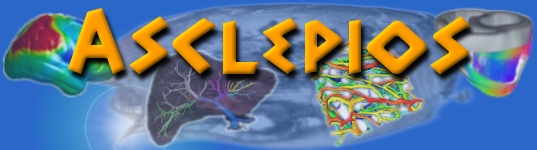
\includegraphics[height=\logoheight]{asclepios-logo.jpg}
 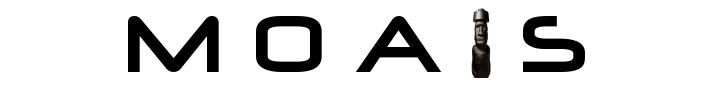
\includegraphics[height=5mm]{moais-logo.png}
\end{center}
%\tableofcontents

\end{frame}

% Etat de l'art
% Linear solutions
% Matrix factoring
% Tree
% layered models
% Extended tree
% Matrix-vector product in etended trees

\section{Motivation}

\begin{frame}
\frametitle{A complex physical simulation}
\begin{center}
 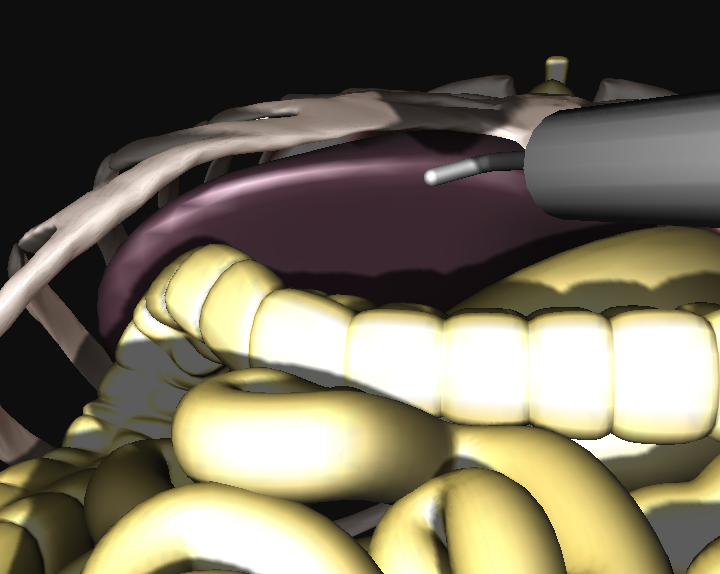
\includegraphics[width=0.7\linewidth]{sofa-laparoscopy1.png}
\end{center}
Material, internal forces, contraints, contact detection and modeling, ODE solution, visualization, interaction, etc.
\end{frame}

%----------------------------------------------------
\begin{frame}
\frametitle{Open-Source Simulation Software}
\newcommand{\himg}{0.25\linewidth}
\begin{tabular}{ccc}
 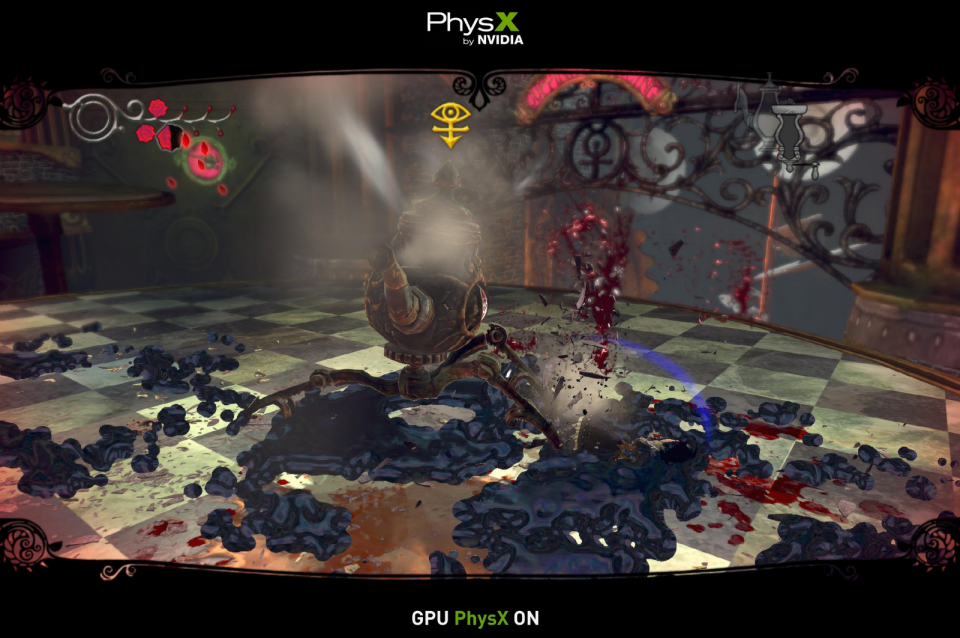
\includegraphics[height=\himg]{physx-Alice-EyepotParticlesFluid.png} & 
 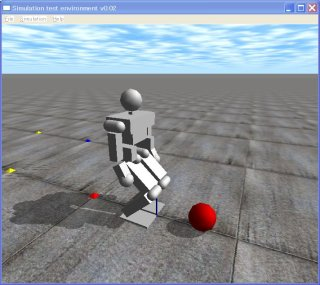
\includegraphics[height=\himg]{ode-humanoid2.jpg} & 
 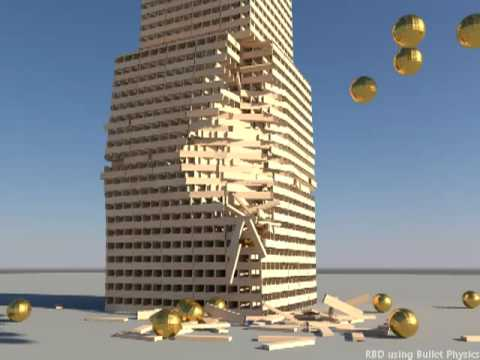
\includegraphics[height=\himg]{bulletphysics-hqdefault.jpg} \\
 PhysX & ODE & Bullet
\end{tabular}

\begin{itemize}
\item Open-source libraries (ODE, Bullet, PhysX, etc.) provide:
\begin{itemize}
\item limited number of material types
\item limited number of geometry types
\item no control on collision detection algorithms
\item no control on interaction modeling
\item few (if any) control of the numerical models and methods.
\item no control on the main loop
%\item few (if any) parallelism
\end{itemize}
\item We need much more !
\begin{itemize}
 \item models, algorithms, scheduling, visualization, etc.
\end{itemize}

\end{itemize}
\end{frame}


%----------------------------------------------------
\begin{frame}
\frametitle{A generic approach}
\begin{itemize}
\item Behavior model: all internal laws
\item Others: interaction with the world
\item Mappings: relations between the models (uni- or bi-directional)
\end{itemize}
\begin{center}
 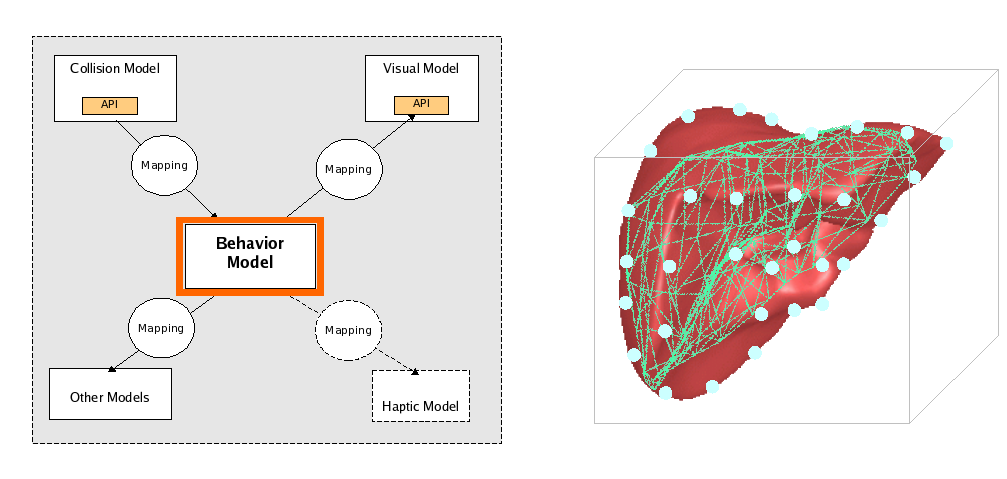
\includegraphics[width=\linewidth]{multimodal.png}
\end{center}

\end{frame}



%-----------------------------------------
\begin{frame}[fragile]
\frametitle{Animation of a simple body}
\begin{columns}

\column[t]{0.5\linewidth}
\begin{itemize}
\item a liver
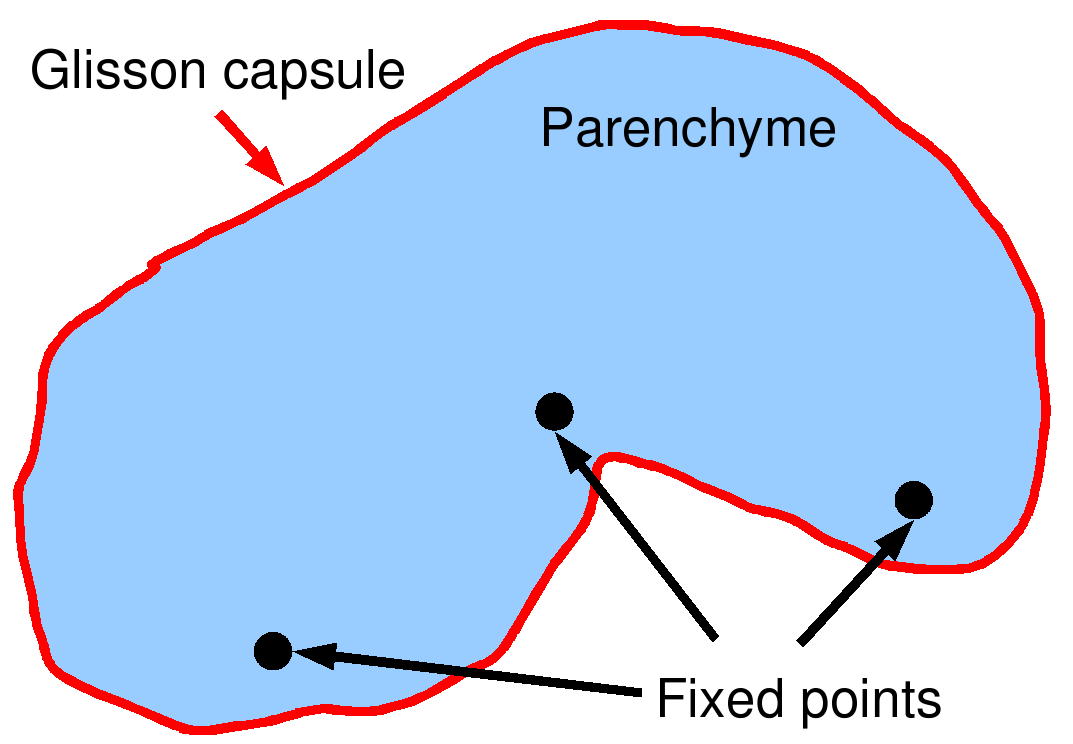
\includegraphics[width=\linewidth]{liver_2ForceFields.png}
\item inside: soft material
\item surface: stiffer material
\end{itemize}

\column[t]{0.5\linewidth}
A specialized program:
\lstset{basicstyle=\large}
\begin{code_cpp}
f = M*g
f += F1(x,v)
f += F2(x,v)
a = f/M
a = C(a)
v += a * dt
x += v * dt
display(x)
\end{code_cpp}

\end{columns}

\end{frame}





%%%==================================================================
\section{Simple bodies}
%%%==================================================================


%-----------------------------------------
\begin{frame}
\frametitle{Components}
\begin{columns}
 \column[c]{0.5\linewidth}
%Data:
\begin{itemize}
\item<1-> state vectors (DOF): $x,v,a,f$
\item<1-> constraints: fixed points 
\only<1> {\\ \em other: oscillator, collision plane, etc.}
\item<2-> force field: tetrahedron FEM
\only<2> {\\ \em other: triangle FEM, springs, Lennard-Jones, SPH, etc.}
\item<3-> force field: triangle FEM
\item<4-> mass: uniform
\only<4> {\\ \em other: diagonal, sparse symmetric matrix}
\item<5-> ODE solver: explicit Euler
\only<5> {\\ \em other: Runge-Kutta, implicite Euler, static solution, etc.}
\end{itemize}
 \column[c]{0.5\linewidth}
\only<1>{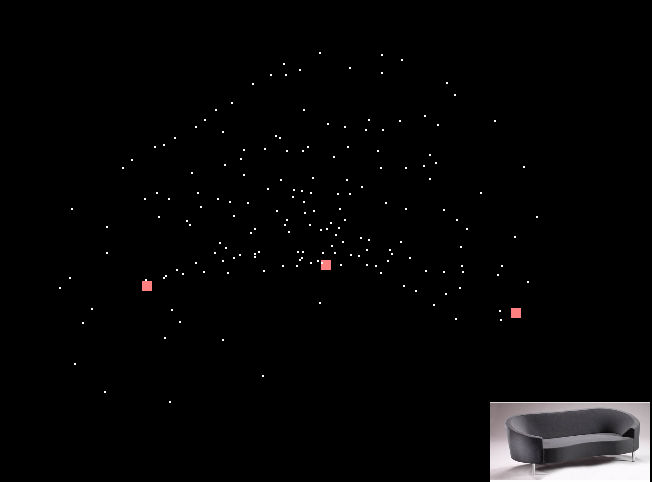
\includegraphics[width=0.9\linewidth]{liverDOF.png}\\ 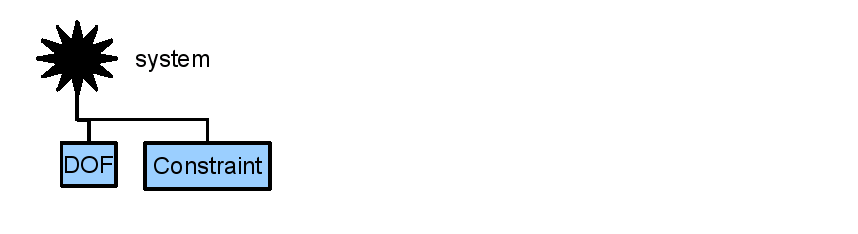
\includegraphics[width=\linewidth]{layeredLiver3-tree-1.png}}
\only<2>{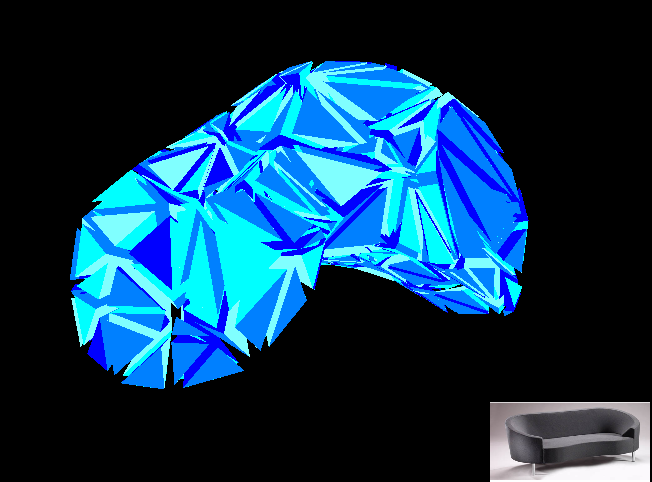
\includegraphics[width=0.9\linewidth]{liverTetra.png}\\ 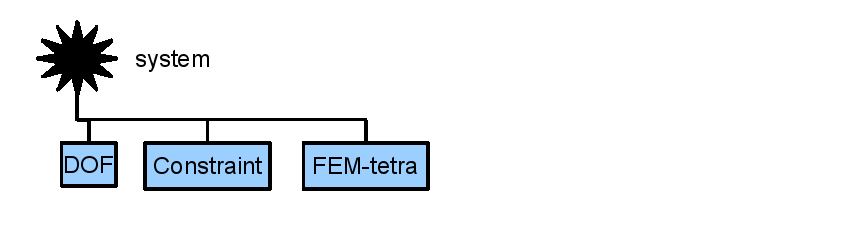
\includegraphics[width=\linewidth]{layeredLiver3-tree-2.png}}
\only<3>{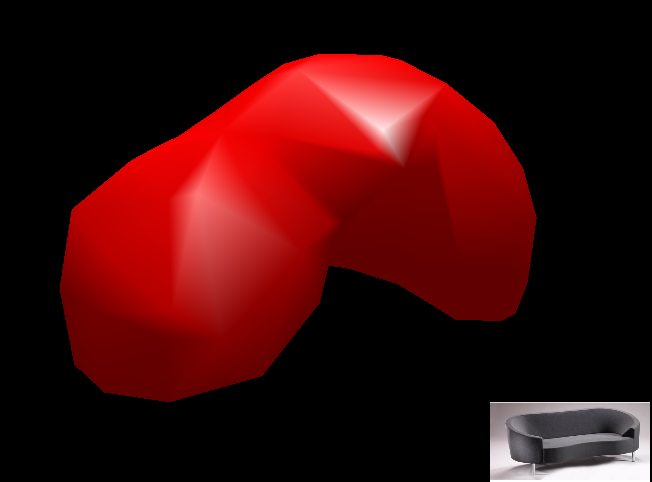
\includegraphics[width=0.9\linewidth]{liverTrian.png}\\ 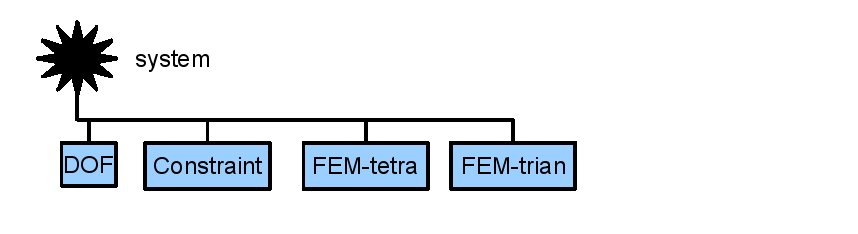
\includegraphics[width=\linewidth]{layeredLiver3-tree-3.png}}
\only<4>{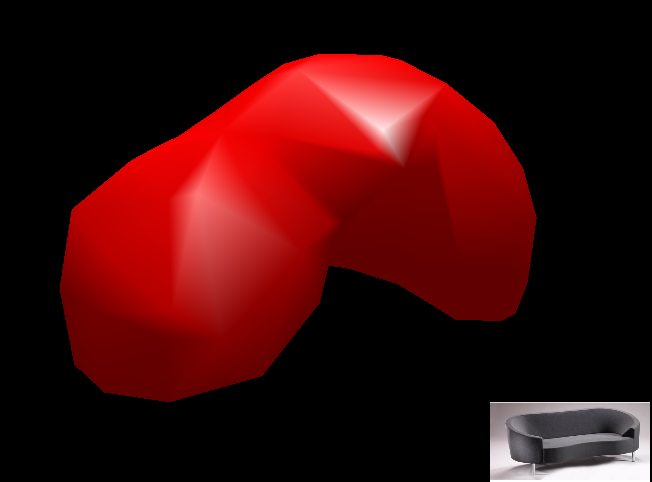
\includegraphics[width=0.9\linewidth]{liverTrian.png}\\ 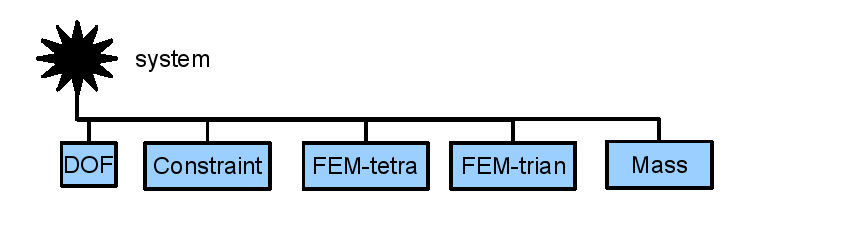
\includegraphics[width=\linewidth]{layeredLiver3-tree-4.png}}
\only<5>{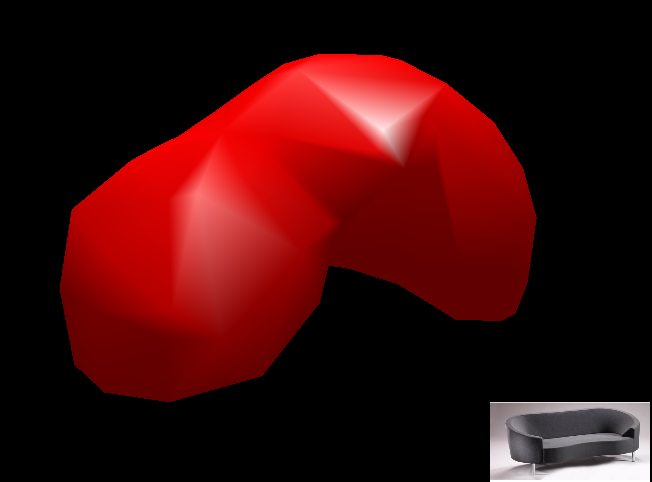
\includegraphics[width=0.9\linewidth]{liverTrian.png}\\ 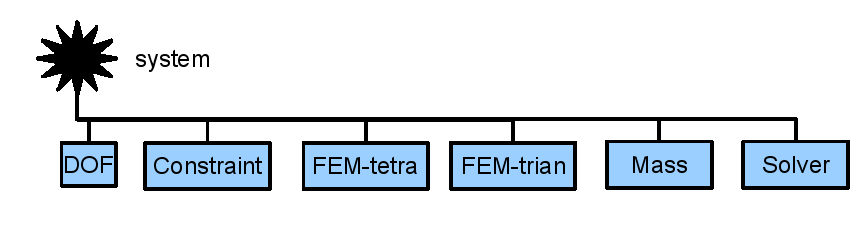
\includegraphics[width=\linewidth]{layeredLiver3-tree-5.png}}
\end{columns}
\end{frame}


%-----------------------------------------
\begin{frame}
\frametitle{Multiple objects with their own solvers}
Each object can be simulated using its own solver

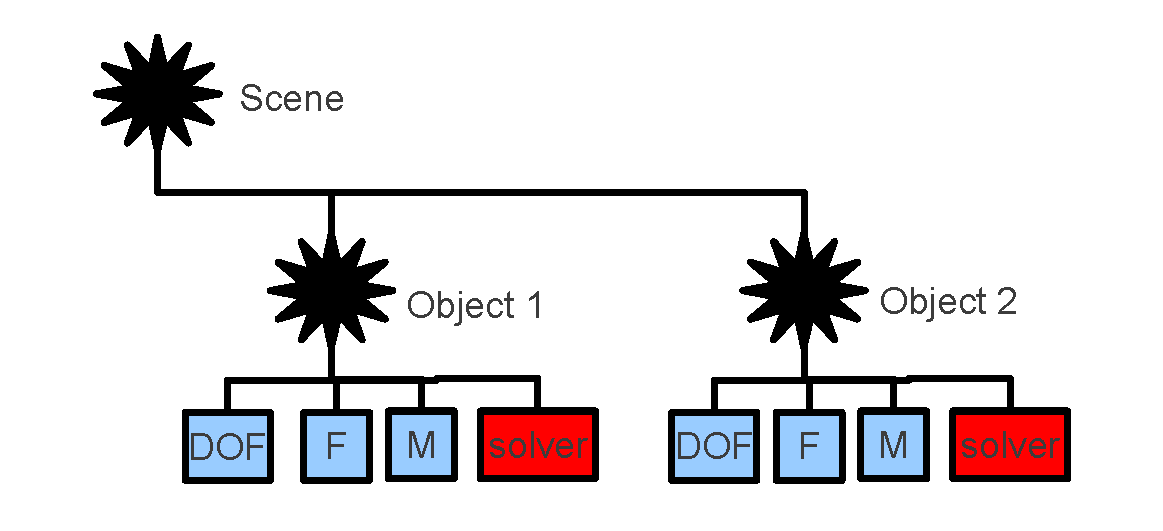
\includegraphics[page=1,width=0.9\linewidth]{solvers.pdf}
\end{frame}

%-----------------------------------------
\begin{frame}
\frametitle{Multiple objects with the same solver}
A solver can drive an arbitrary number of objects of arbitrary types

\includegraphics[page=2,width=0.9\linewidth]{solvers.pdf}
\end{frame}



%-----------------------------------------
\begin{frame}
\frametitle{Processing multiple objects using visitors}

\begin{itemize}
 \item The ODE solver sends visitors to apply operations
 \item The visitors traverse the scene and apply virtual methods to the components
 \item The methods read and write state vectors (identified by symbolic constants) in the DOF component
 %\item State vectors are identified by symbolic constants 
 \item Example: accumulate force
  \begin{itemize}
   \item A \texttt{ResetForceVisitor} recursively traverses the nodes of the scene (only one node here)
  \begin{itemize}
   \item All the \texttt{DOF} objects apply their \texttt{resetForce()} method
  \end{itemize}
   \item An \texttt{AccumulateForceVisitor} recursively traverses the nodes of the scene 
  \begin{itemize}
   \item All the \texttt{ForceField} objects apply their \texttt{addForce(  Forces, const Positions, const Velocities )} method
  \end{itemize}
   \item the final value of f is weight + tetra fem force + trian fem force
  \end{itemize}
\end{itemize}

\end{frame}



%-----------------------------------------
\begin{frame}
\frametitle{Scene data structure}

Scene hierarchy:
\begin{enumerate}
 \item the scene is composed of \textit{nodes} organized in a Directed Acyclic Graph (DAG, i.e. generalized hierarchy)
 \item nodes contain \textit{components} (mass, forces, etc.)  and a list of child nodes
 \item components contain \textit{attributes} (density, stiffness, etc.)
\end{enumerate}

Data graph:
\begin{itemize}
 \item attributes can be connected together for automatic copies
 \item attributes can be connected by \textit{engines}, which update their output based on the values of their input
 \item the attributes and engine compose a DAG
\end{itemize}


\end{frame}




% %-----------------------------------------------
% \begin{frame}[fragile]
% \frametitle{Object-oriented hierarchical structure}
% \begin{columns}
% \column[c]{0.5\linewidth}
% \begin{itemize}
%  \item The system aggregates abstract components
%  \item The components are independent
% \item
%  \only<2>{\item Force fields: springs, triangle FEM, tetrahedron FEM, SPH, etc.}
%  \only<3>{ Constraints: fixed points, oscillators, half-space, etc.}
%  \only<4>{\item Mass: uniform, diagonal, symmetric sparse matrix}
%  \only<5>{\item Solver: explicit Euler, implicit Euler, Runge-Kutta, static, etc. }
% 
%  \item They communicate through the system
%  \item The solver triggers \textit{actions}
% \end{itemize}
% 
%  \column[c]{0.5\linewidth}
% \includegraphics[width=\linewidth]{system_simple.png}
% \end{columns}
% \end{frame}



%%%===================================================================
\section{Layered objects using node hierarchies}
%%%===================================================================

\begin{frame}
\frametitle{Layered object }
Detailed geometry embedded in a coarse deformable grid
\begin{columns}
\column[c]{0.5\linewidth}
\begin{itemize}
\item<1-> independent DOFs (blue)
\item<2-> skin vertices (salmon)
\item<3-> mapping 
\item<4-> collision samples (green)
\item<4-> collision mapping
\item<5-> apply displacements
\begin{enumerate}
\item $v_{skin} = J_{skin} v$
\item $v_{collision} = J_{collision} v_{skin}$
\end{enumerate}
\item<6-> apply forces
\begin{enumerate}
\item $f_{skin} = J_{collision}^T f_{collision}$
\item $f = J_{skin}^T f_{skin}$
\end{enumerate}
\end{itemize}
\column[c]{0.5\linewidth}
%Layered body\\
\only<1>{
	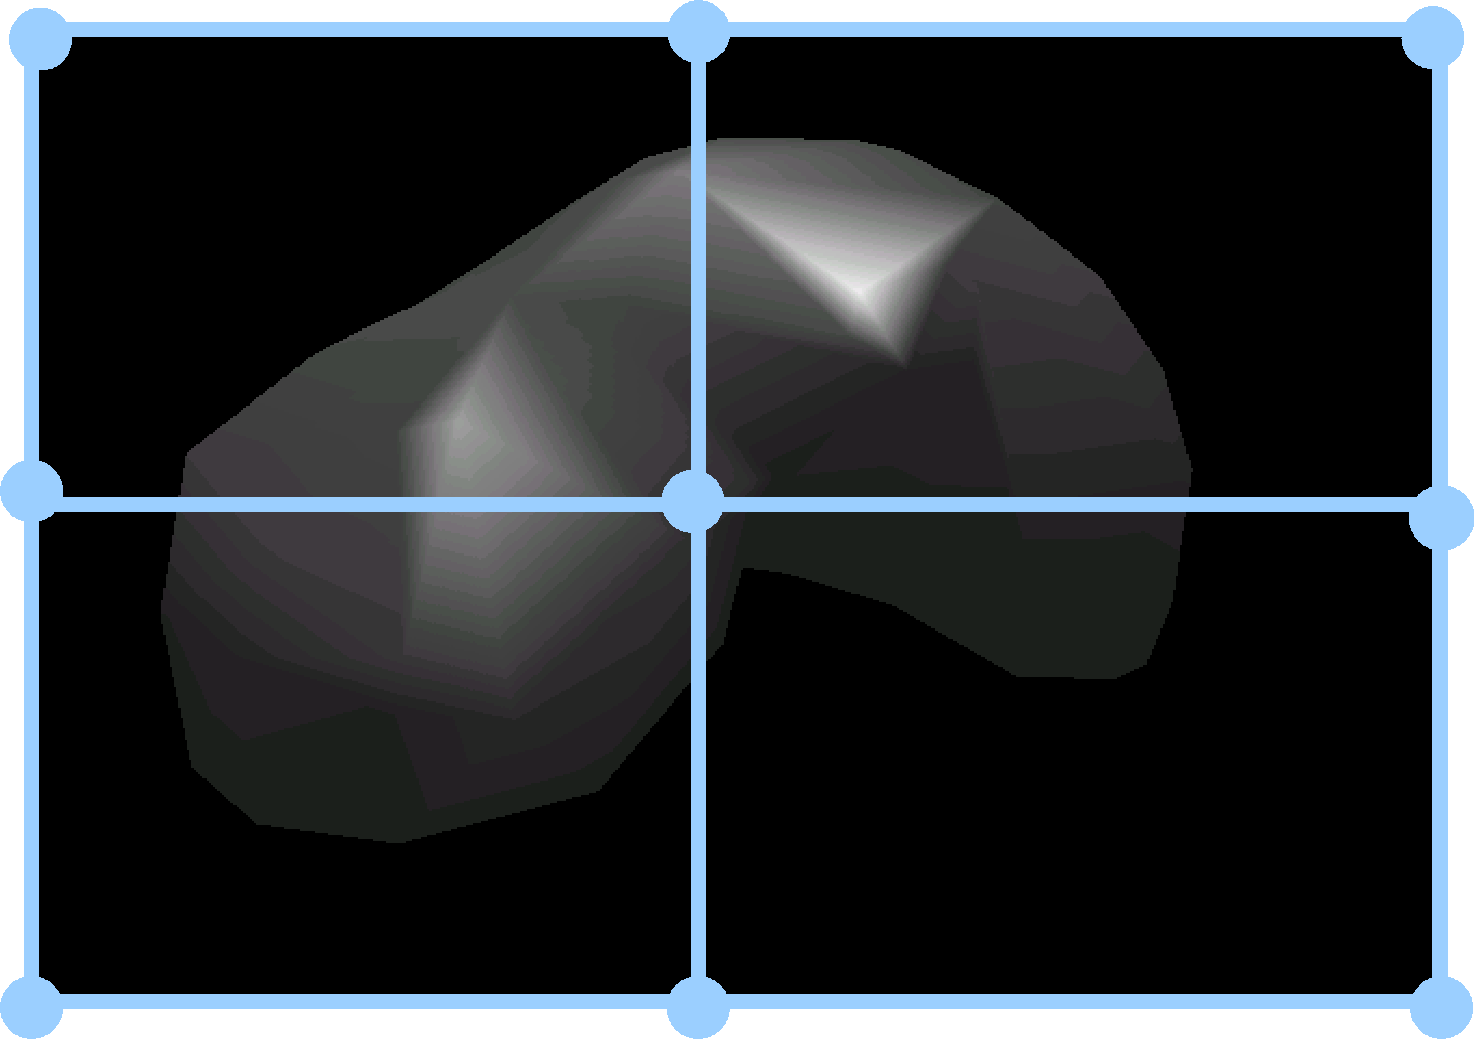
\includegraphics[width=0.8\linewidth]{layeredLiver-bm.png}\\ 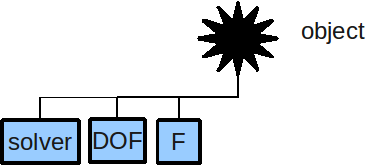
\includegraphics[width=\linewidth]{layered-tree2-1.png}
}
\only<2>{
	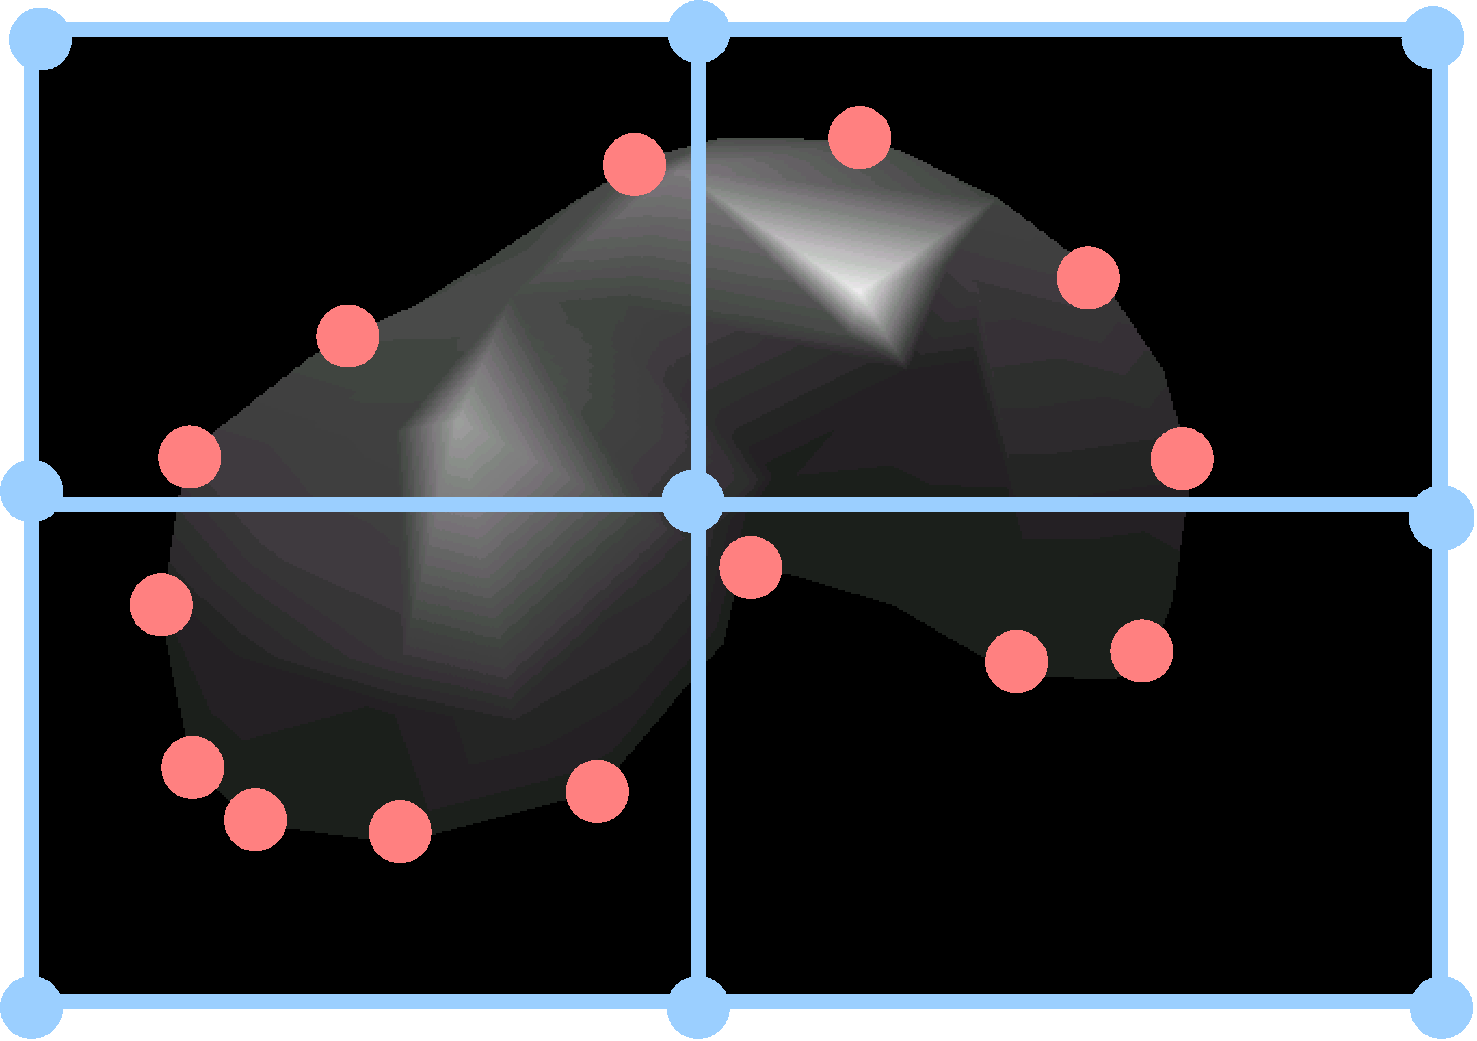
\includegraphics[width=\linewidth]{layeredLiver-bm-vmod.png}\\
	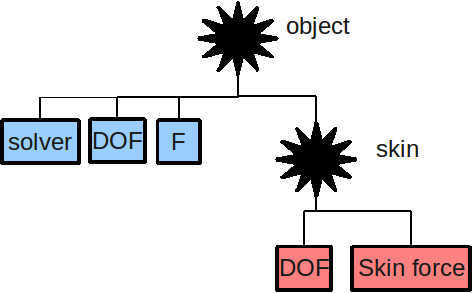
\includegraphics[width=\linewidth]{layered-tree2-2.png}
}
\only<3>{
	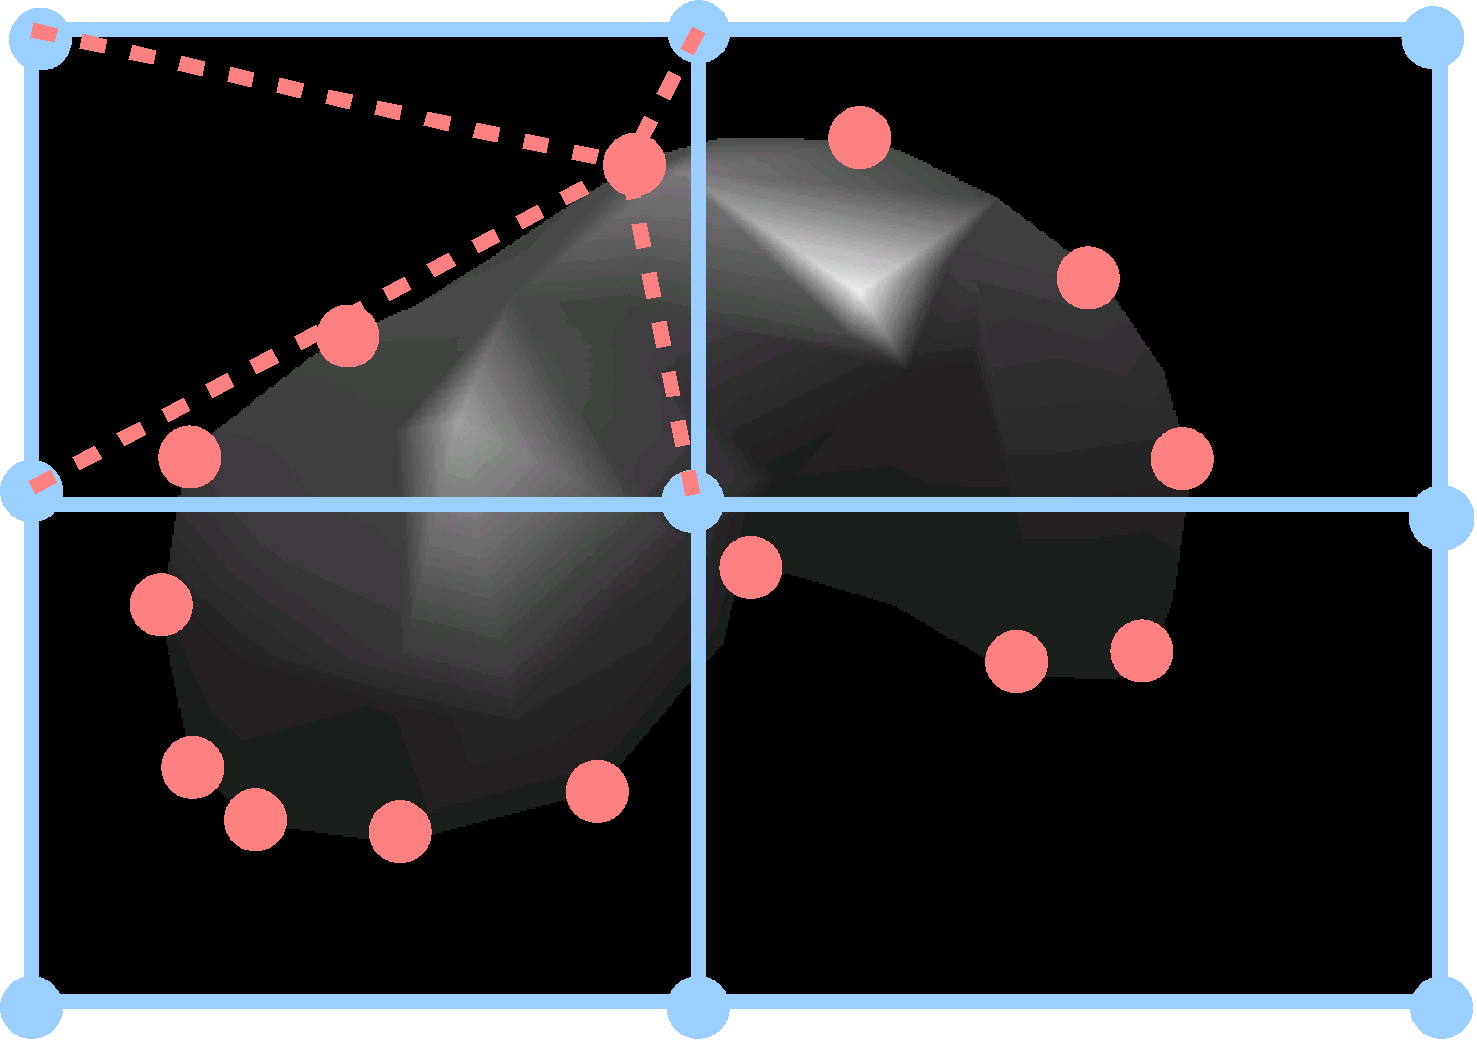
\includegraphics[width=\linewidth]{layeredLiver-bm-vmod-vmap.png}\\
	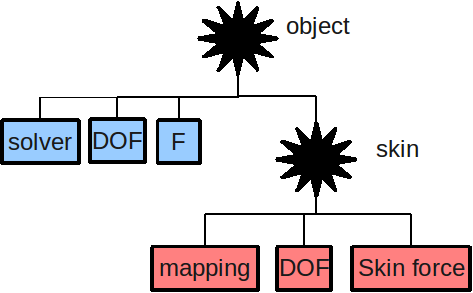
\includegraphics[width=\linewidth]{layered-tree2-3.png}
}
\only<4>{
	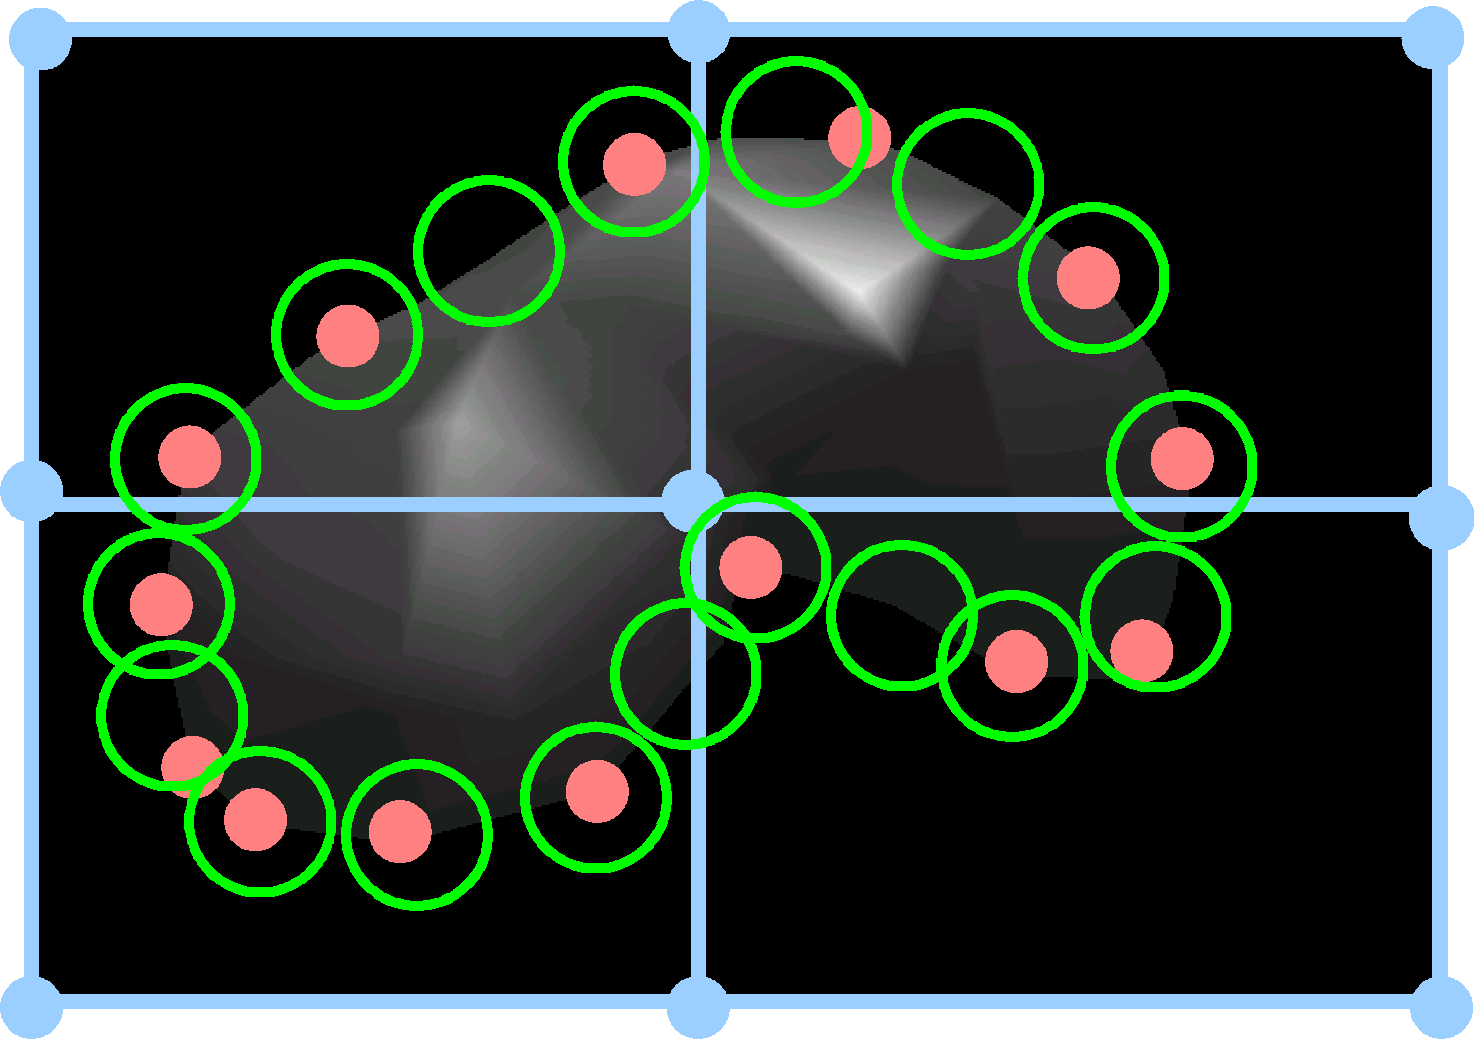
\includegraphics[width=\linewidth]{layeredLiver-bm-vmod-cmod.png}\\
	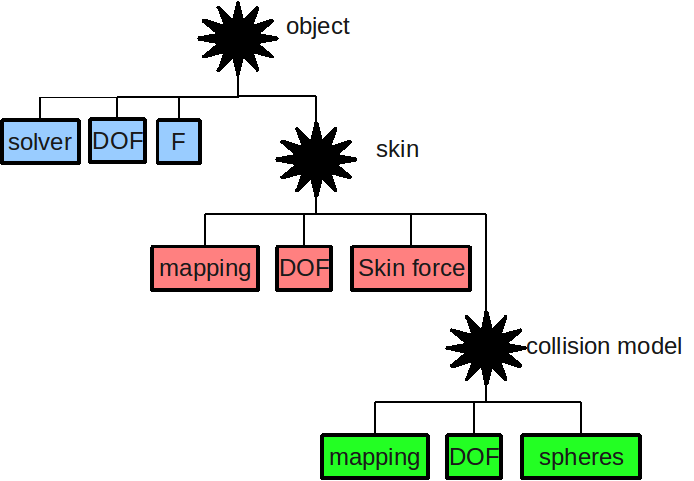
\includegraphics[width=\linewidth]{layered-tree2-4.png}
}
%\only<5>{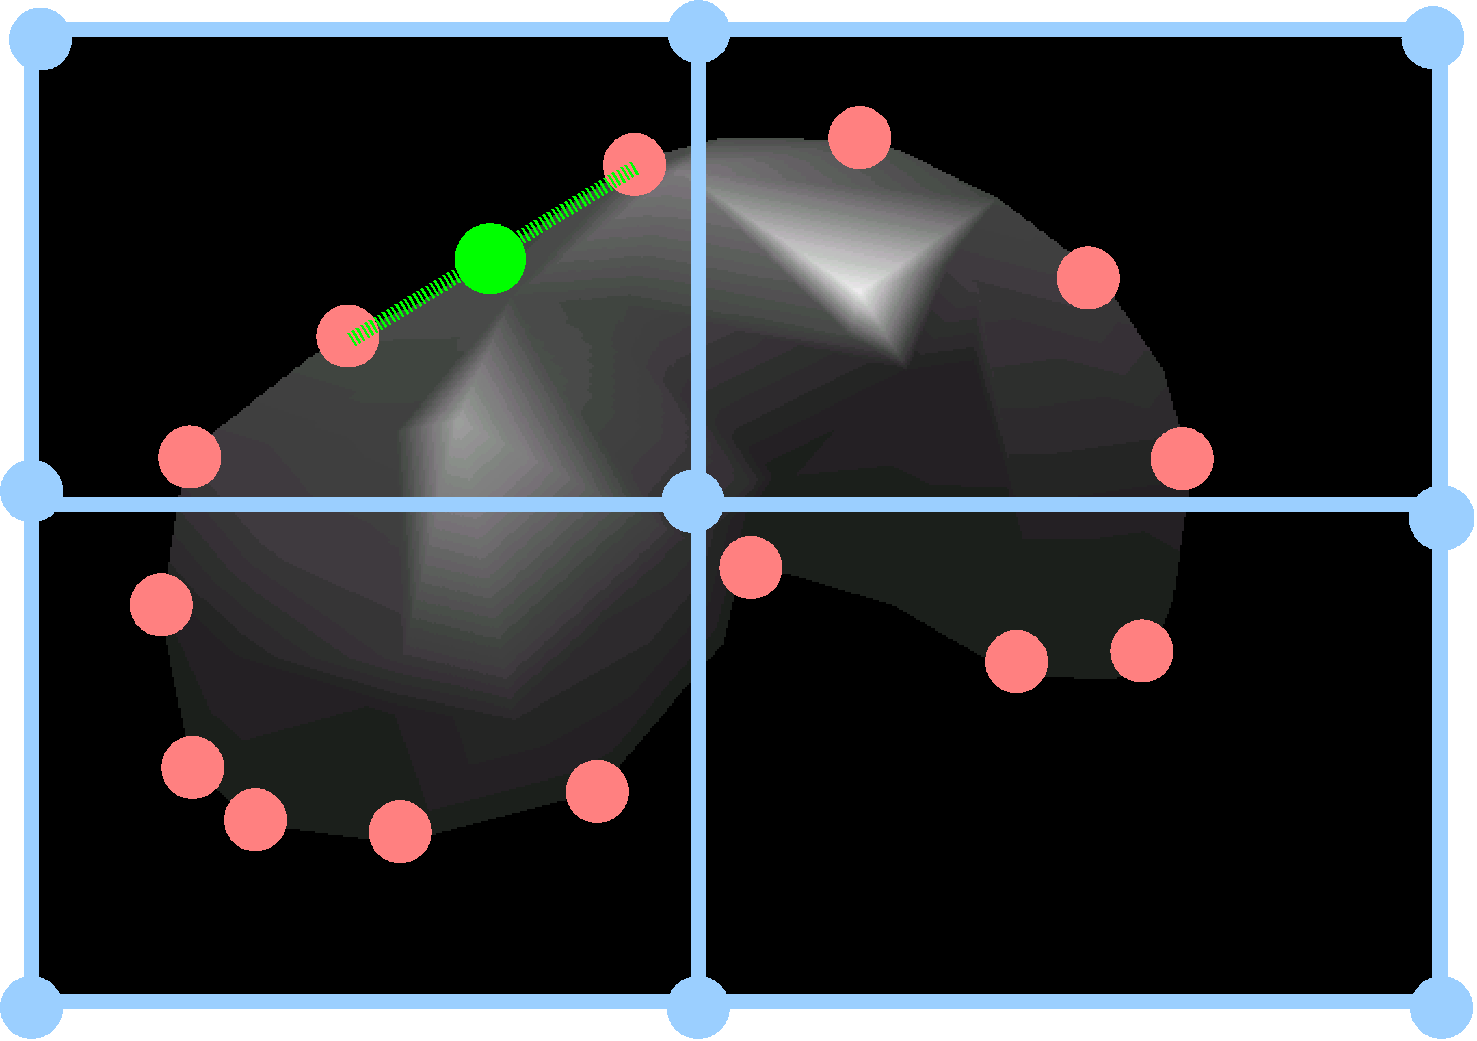
\includegraphics[width=\linewidth]{layeredLiver-bm-vmod-cmap.png}}
\only<5>{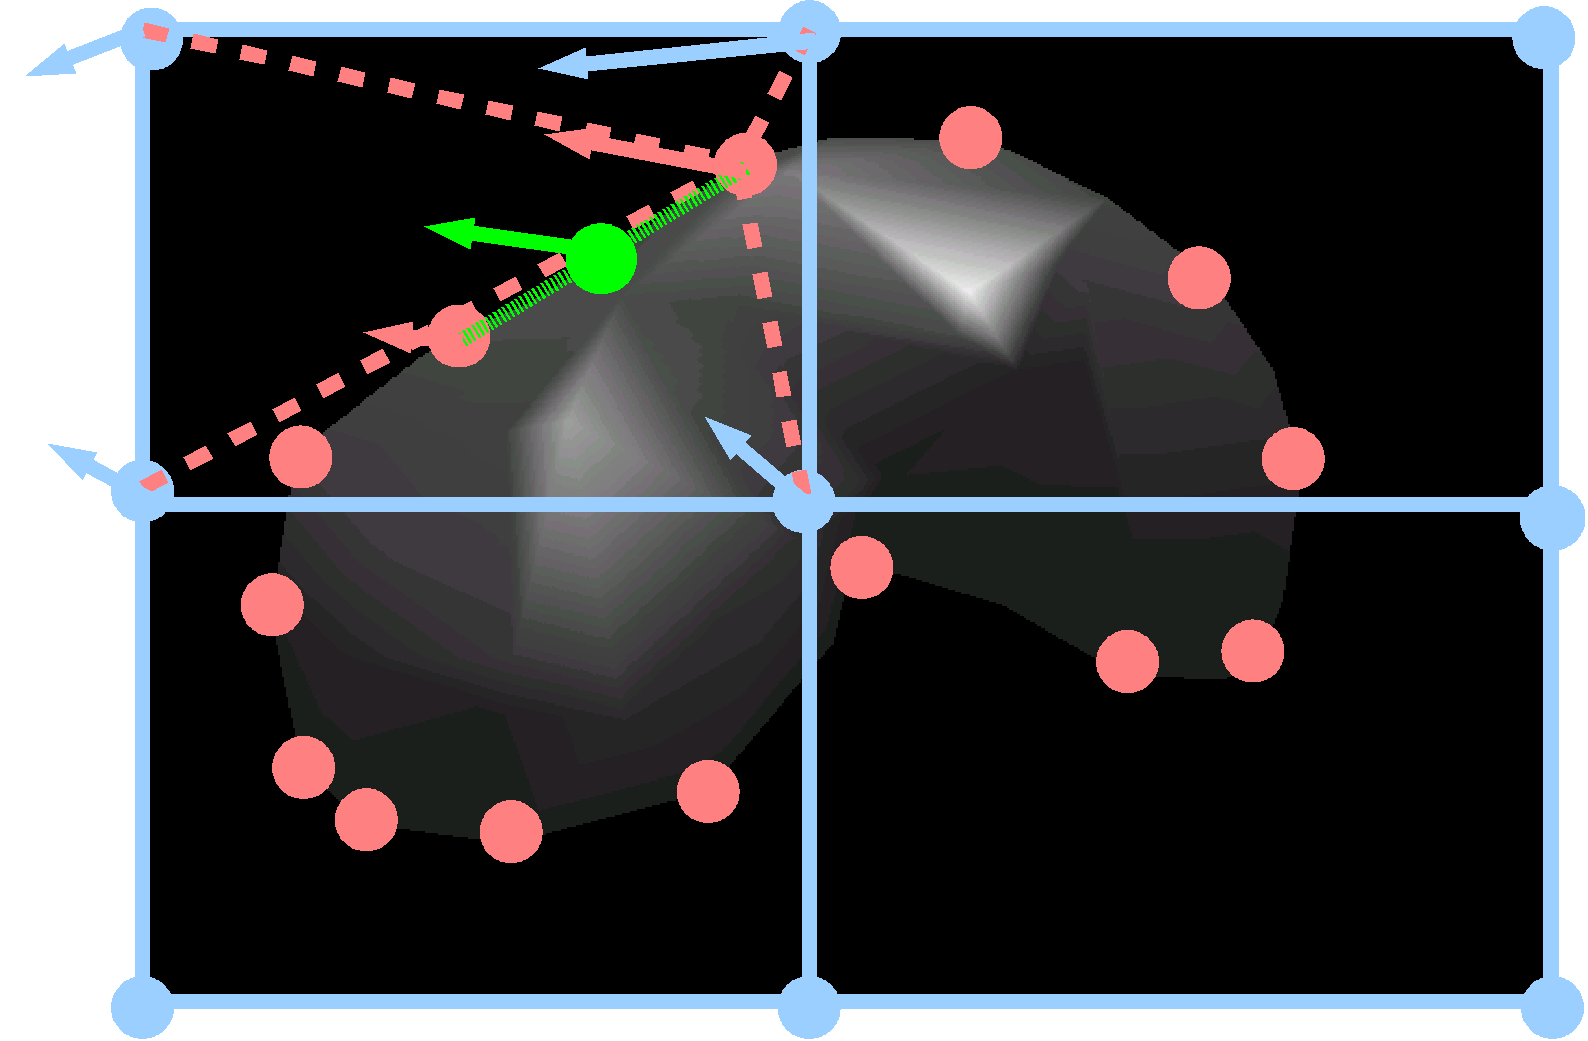
\includegraphics[width=\linewidth]{layeredLiver-v.png}}
\only<6>{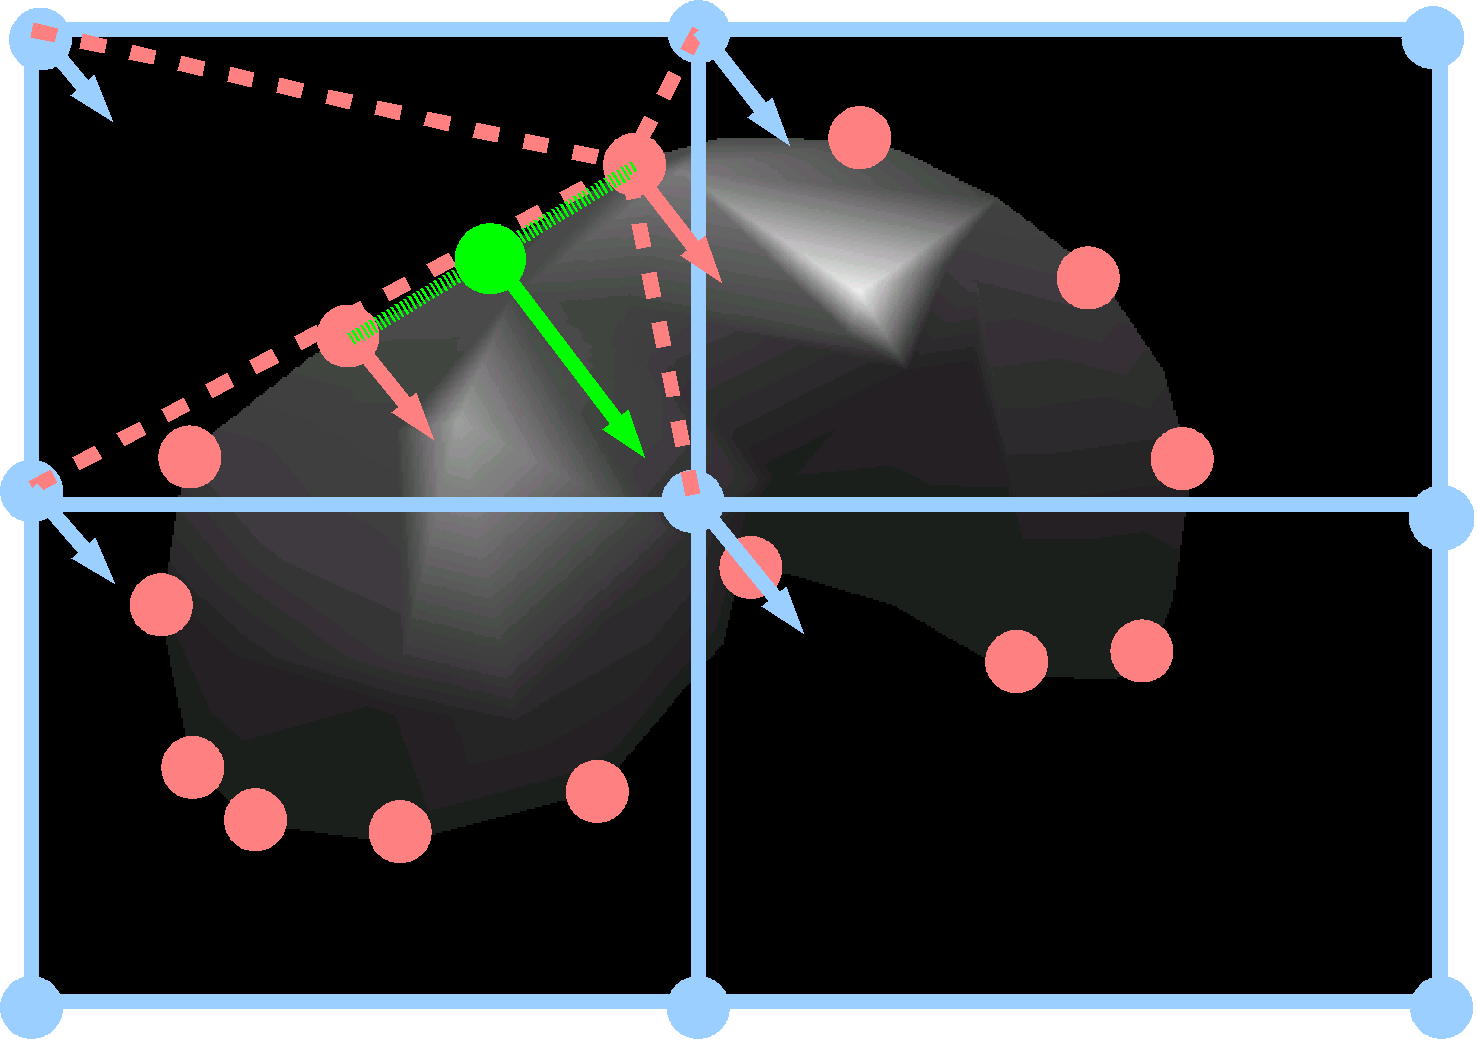
\includegraphics[width=\linewidth]{layeredLiver-f.png}}
\end{columns}
\end{frame}

% %-----------------------------------------------
% \begin{frame}
% \frametitle{Tree processing}
% \begin{columns}
% \column[c]{0.5\linewidth}
% Tree structure:\\
% \includegraphics[width=\linewidth]{layered-tree.png}
% \column[c]{0.5\linewidth}
% Traversals:
% \begin{itemize}
% \item Top-down: propagate positions, velocities, displacements
% \item compute the forces
% \item Bottom-up: sum up the forces 
% \end{itemize}
% \end{columns}
% \end{frame}




% ===================================================================
% \subsection{Mappings}
% ===================================================================

\begin{frame}
\frametitle{More on mappings}
\begin{itemize}
 \item Map a set of degrees of freedom (the parent) to another (the child).
 \item Typically used to attach a geometry to control points (but see Flexible and Compliant plugins).
 \item Child degrees of freedom (DOF) are not independent: their positions are totally defined by their parent's.
 \item Displacements are propagated top-down (parent to child): $v_{child} = Jv_{parent}$
 \item Forces are accumulated bottom-up: $f_{parent} += J^T f_{child}$
%  \item A necessary condition for physical consistency is to induce no energy. This is true iff: $v_{child} = Jv_{parent} \Rightarrow f_{parent} += J^T f_{child}$
%  \item Other physical constraints are not automatically satisfied, e.g. incompressibility of the child
\end{itemize}

\end{frame}


\begin{frame}
\frametitle{The physics of mappings}
Example: line mapping

% 	\begin{center}
% 	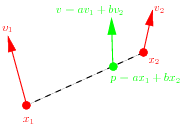
\includegraphics[width=O.3\linewidth]{lineMapping-v.png}
% 	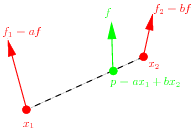
\includegraphics[width=O.3\linewidth]{lineMapping-f.png}
% 	\end{center}
\begin{columns}
\column{0.5\linewidth}
$$
\begin{array}{rcl}
v_c = \left(
\begin{array}{cc}
a & b
\end{array}
\right)
\left(
\begin{array}{c}
v_1 \\ 
v_2
\end{array}
\right)
&=& J v
 \\
\left(\begin{array}{c}
f_1 \\ f_2
\end{array}
\right)
= 
\left(\begin{array}{c}
a \\ 
b
\end{array}
\right)
f_c
&=& J^T f_c
\end{array}
$$
\column{0.5\linewidth}
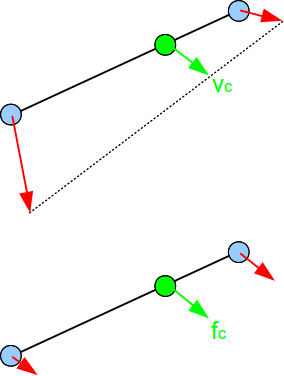
\includegraphics[width=\linewidth]{mapping-force.png}
\end{columns}
\end{frame}


\begin{frame}
\frametitle{Examples of mappings}
\begin{columns}
\column[t]{0.5\linewidth}
\begin{itemize}
 \item<1-> RigidMapping can be used to attach points to a rigid body
 \only<1-2>{
  \begin{itemize}
  \only<1>{\item to attach a visual model }
  \only<2>{ \item to attach collision surfaces }
 \end{itemize}
 }

 \item<3-> BarycentricMapping can be used to attach points to a deformable body
\only<3-4>{
\begin{itemize}
 \only<3>{\item to attach a visual model }
 \only<4>{\item to attach collision surfaces }
\end{itemize}
}

\item<5-> More advanced mapping can be applied to fluids

\end{itemize}
\column[T]{0.5\linewidth}
\only<1>{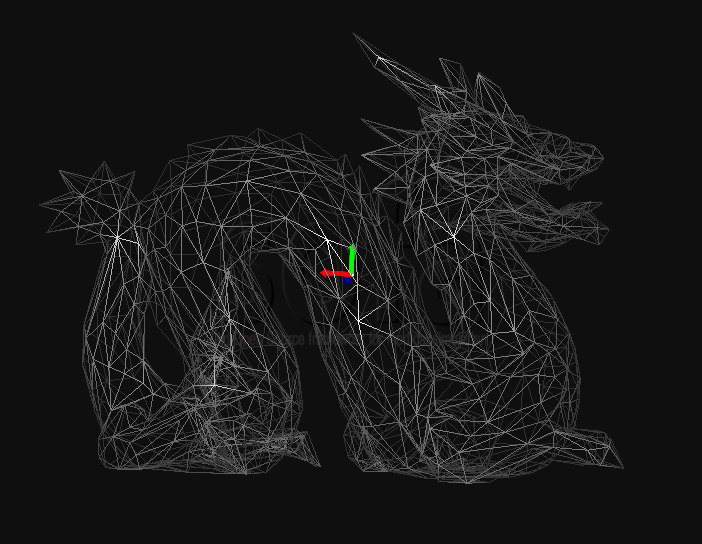
\includegraphics[width=\linewidth]{dragon-wire.png} \\ 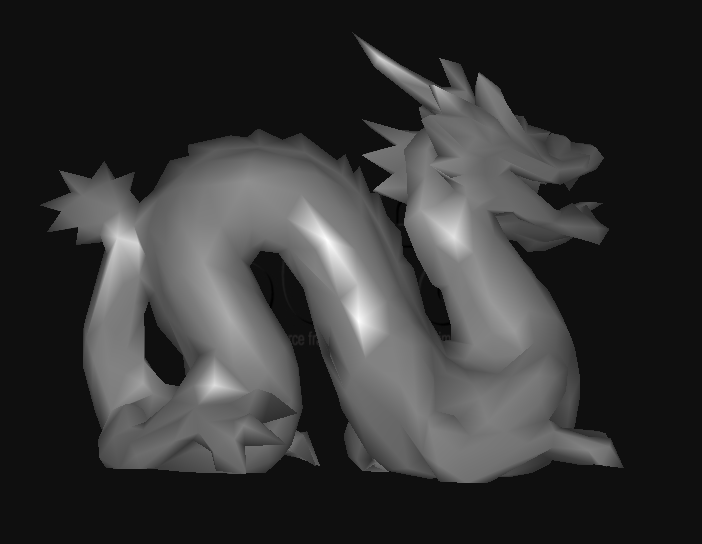
\includegraphics[width=\linewidth]{dragon-plain.png}}
\only<2>{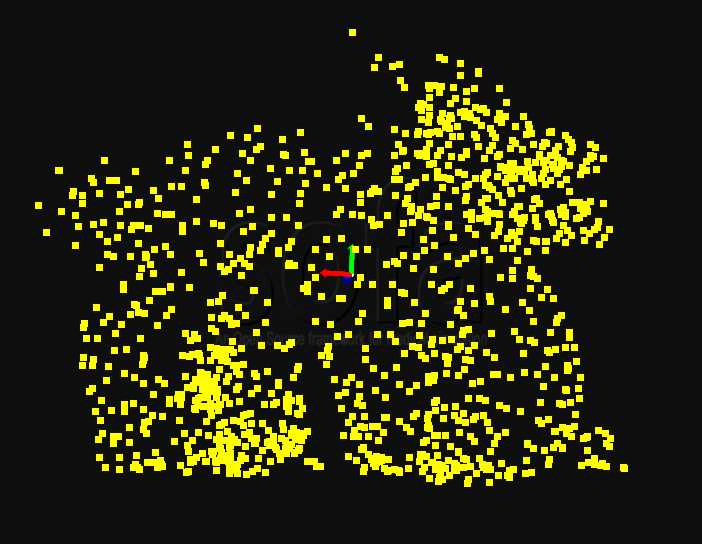
\includegraphics[width=\linewidth]{dragon-spheres-mapping.png} \\ 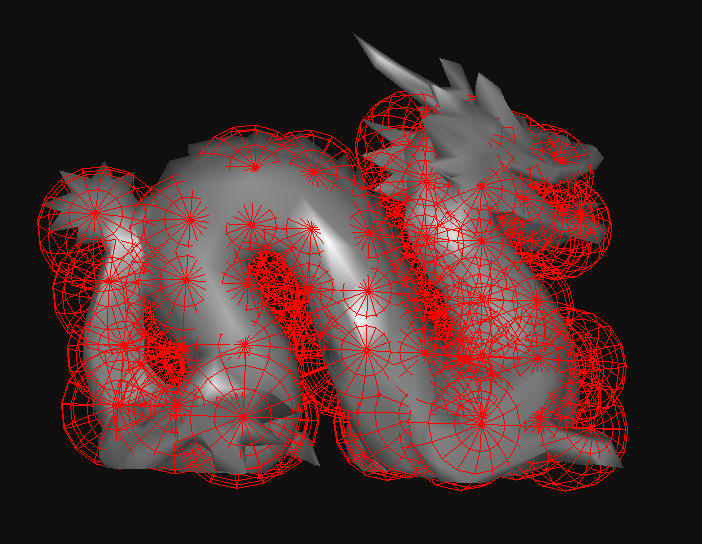
\includegraphics[width=\linewidth]{dragon-spheres.png}}
% \only<3>{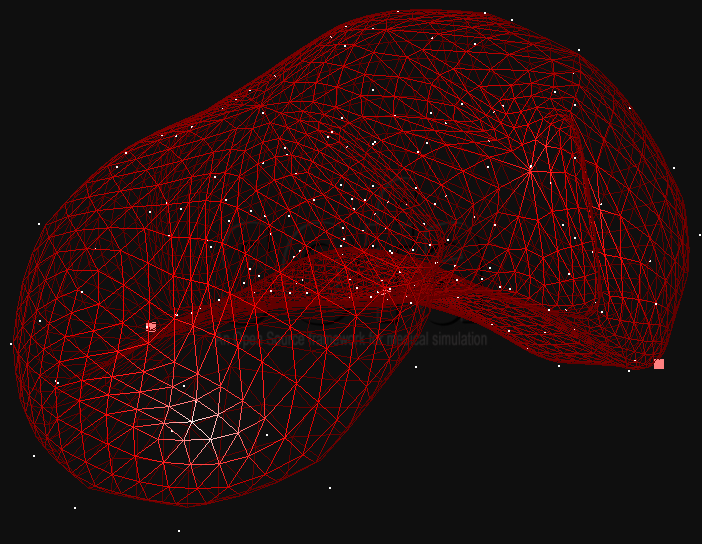
\includegraphics[width=\linewidth]{liver-wire.png} \\ 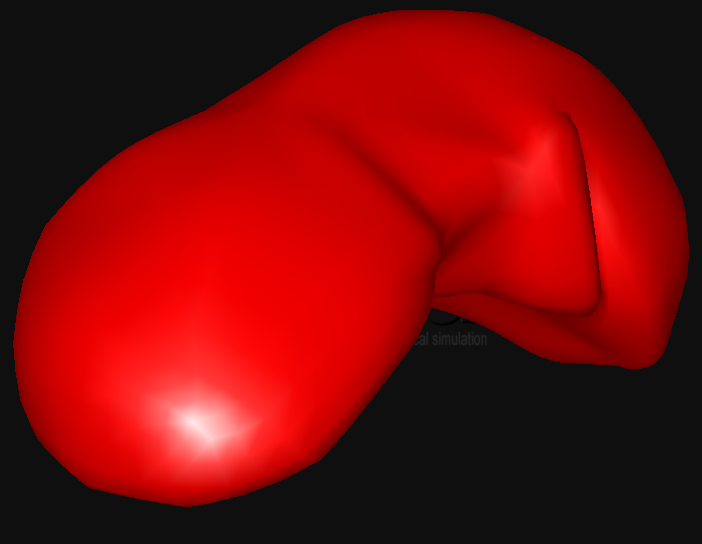
\includegraphics[width=\linewidth]{liver-plain.png}}
\only<3>{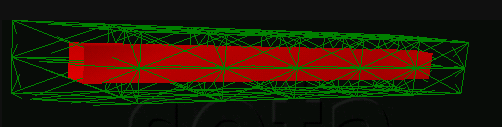
\includegraphics[width=\linewidth]{bary-init.png} \\ 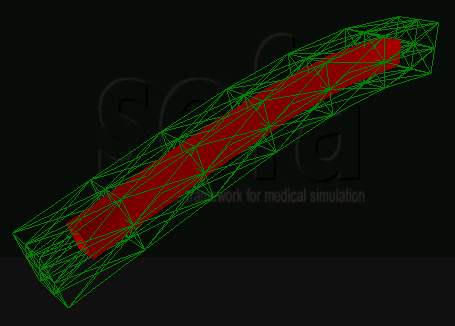
\includegraphics[width=\linewidth]{bary-deformed.png}}
\only<4>{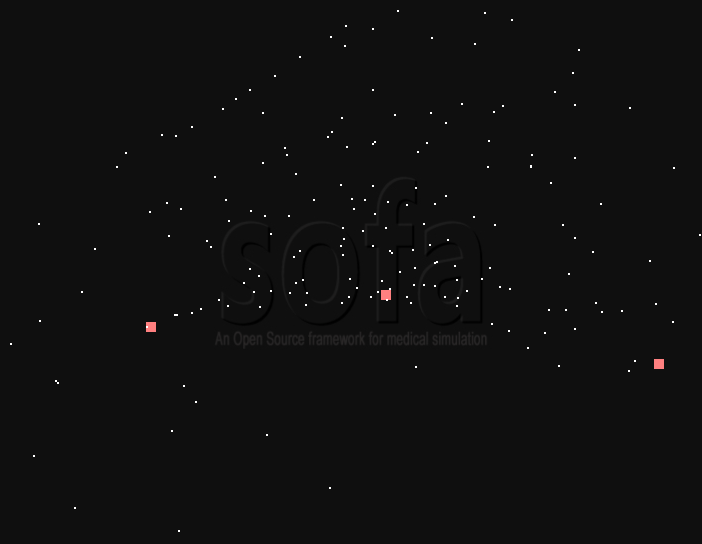
\includegraphics[width=\linewidth]{liver-dof.png} \\ 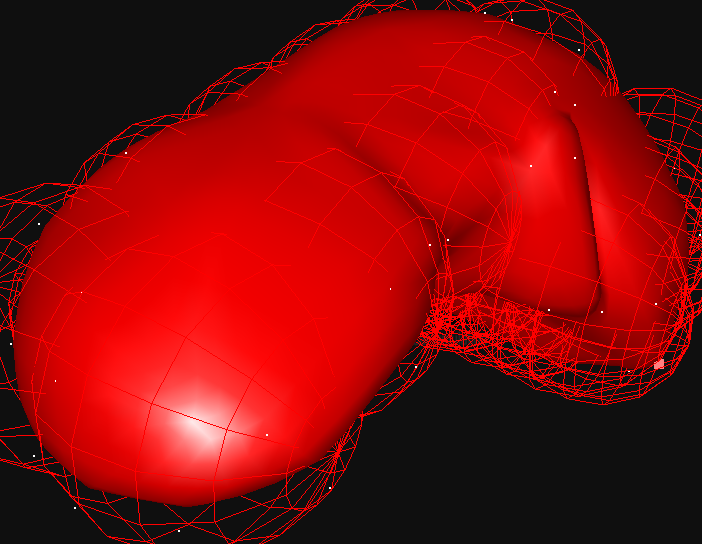
\includegraphics[width=\linewidth]{liver-spheres.png}}
\only<5>{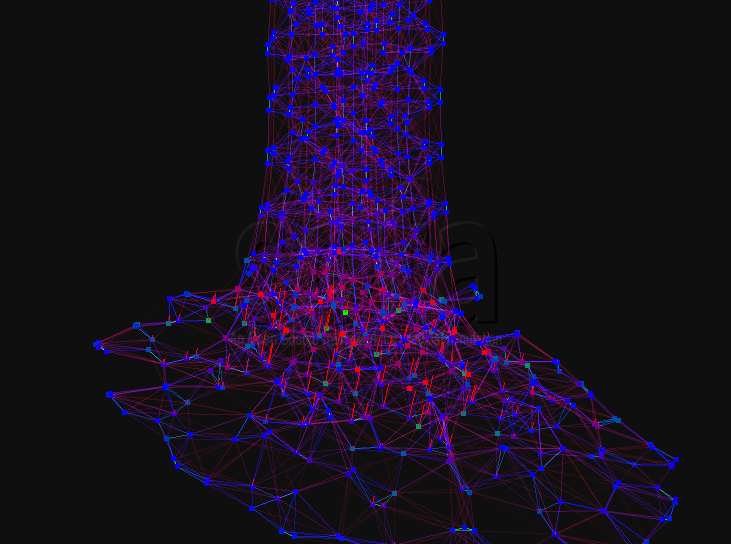
\includegraphics[width=\linewidth]{sph-force.png} \\ \includegraphics[width=\linewidth]{sph-plain.png}}
\only<6>{\includegraphics[width=\linewidth]{sph-dof.png} \\ \includegraphics[width=\linewidth]{sph-mapping.png}}
\end{columns}

\end{frame}

\begin{frame}
\frametitle{On the physical consistency of mappings}
\begin{itemize}
 \item Conservation of energy:\\Necessary condition: $v_{child} = Jv_{parent} \Rightarrow f_{parent} += J^T f_{child}$
 \item Conservation of momentum:\\
 Mass is modeled at one level only. There is no transfer of momentum.
 \item Constraints on displacements (e.g. incompressibility, fixed points) are not easily applied \textit{at the child level}
\end{itemize}

\end{frame}



%%%===================================================================
\section{Interacting objects}
%%%===================================================================

\begin{frame}
\frametitle{Two objects in contact}
Example: 2-layer liver against 3-layer liver using a contact force.\\
Use extended trees (Directed Acyclic Graphs) to model trees with loops.
\begin{columns}
\column{0.3\linewidth}
\includegraphics[width=\linewidth]{livers-contact.png}
\column{0.7\linewidth}
\includegraphics[width=\linewidth]{livers-contact-tree.png}
\end{columns}
\end{frame}


%-----------------------------------------------
\begin{frame}
\frametitle{ODE solution of interacting objects}
 \only<1>{\includegraphics[width=0.9\linewidth]{livers-contact-tree-independent.png}}
 \only<2->{\includegraphics[width=0.9\linewidth]{livers-contact-tree-common.png}}
\begin{itemize}
\item<1-> Soft interactions: independent processing, no synchronization required\\
\item<2-> Stiff interactions: unified implicit solution with linear solver, synchronized objects\\
\item<3-> Hard interaction constraints using Lagrange multipliers 
\end{itemize}
\end{frame}




%%%===================================================================
\section{Implementation}
%%%===================================================================


\begin{frame} 
\frametitle{Actions implemented by Visitors}
\begin{center}
 \includegraphics[width=0.7\linewidth]{livers-contact-tree-common.png}
\end{center}


\begin{itemize}
\item No global state vector
% \begin{itemize}
%  \item they are scattered over the DOF components
%  \item each DOF component can be based on its own types (e.g. Vec3, Frame, etc. )
%  \item symbolic values are used to represent global state vectors
% \end{itemize}
 \item Operation = graph traversal + abstract methods + vector identificators
% \begin{itemize}
%  \item Displacements are propagated top-down
%  \item Interactions forces are evaluated after displacement propagation
%  \item Forces are accumulated bottom-up
%  \item Branches can be processed in parallel
% \end{itemize}

\end{itemize}

\end{frame}


%-----------------------------------------------

\begin{frame}
 \frametitle{Example: clearing a global vector}
\begin{itemize}
 \item The solver triggers an action starting from its parent system and carrying the necessary symbolic information
\item the action is propagated through the graph and calls the appropriate methods at each DOF node
\end{itemize}
\begin{center}
 \includegraphics[width=0.8\linewidth]{layered-contacts-action-resetF.png}
\end{center}

\end{frame}


% %-----------------------------------------------
% 
% \begin{frame}
%  \frametitle{Example: applying interaction forces}
% \begin{itemize}
%  \item The solver triggers the appropriate action
% \item the action is propagated through the graph and calls the appropriate methods at each Contact node
% \end{itemize}
% \begin{center}
%  \includegraphics[width=0.8\linewidth]{layered-contacts-action-applyInteractionForces.png}
% \end{center}
% 
% \end{frame}


%-----------------------------------------------

\begin{frame}
 \frametitle{Example: accumulating the forces}
\begin{itemize}
 \item The solver triggers the appropriate action
 \item the action is propagated through the graph and calls the appropriate (botom-up) methods at each Force and Mapping node
\end{itemize}
\begin{center}
 \includegraphics[width=0.8\linewidth]{layered-contacts-action-accumulateForces.png}
\end{center}

\end{frame}



% %-----------------------------------------------
% 
% \begin{frame}
%  \frametitle{Example: computing the accelerations}
% \begin{itemize}
%  \item The solver triggers the appropriate action
%  \item the action is propagated through the graph and calls the appropriate methods at each Mass node
% \end{itemize}
% \begin{center}
%  \includegraphics[width=0.8\linewidth]{layered-contacts-action-accumulateForces.png}
% \end{center}
% 
% \end{frame}
% 
% 
% %-----------------------------------------------
% 
% \begin{frame}
%  \frametitle{Example: vector operation}
% \begin{itemize}
%  \item The solver triggers the appropriate action
%  \item the action is propagated through the graph and calls the appropriate methods at each {\em independent} DOF node
% \end{itemize}
% \begin{center}
%  \includegraphics[width=0.8\linewidth]{layered-contacts-action-add.png}
% \end{center}
% 
% \end{frame}


% %-----------------------------------------------
% 
% \begin{frame}
%  \frametitle{Example: state propagation}
% \begin{itemize}
%  \item The solver triggers the appropriate action
%  \item the action is propagated through the graph and calls the appropriate method (top-down) at each mapping node
% \end{itemize}
% \begin{center}
%  \includegraphics[width=0.8\linewidth]{layered-contacts-action-propagateV.png}
% \end{center}
% 
% \end{frame}


%-----------------------------------------------

\begin{frame}
 \frametitle{Efficient implicit integration}
\begin{itemize}
 \item Large time steps for stiff internal forces and interactions
 \item solve $ (\alpha M + \beta h^2 K ) \Delta v = h( f + hKv) $ Iteratively using a conjugate gradient solution
\end{itemize}
 Actions:
\begin{itemize}
 \item propagateDx
 \item computeDf
 \item vector operations
 \item dot product (only global value directly accessed by the solver)
\end{itemize}
System assembly in the Compliant plugin
\end{frame}


\begin{frame}
\frametitle{Efficiency}
% \begin{center}
%  \includegraphics[width=0.4\linewidth]{livers-contact-tree.png}
% \end{center}


\begin{itemize}
\item No global state vector
\begin{itemize}
 \item they are scattered over the DOF components
 \item each DOF component can be based on its own types (e.g. Vec3, Frame, etc. )
 \item symbolic values are used to represent global state vectors
\end{itemize}
 \item Action = graph traversal + global vector ids + call of abstract top-down and bottom up methods 
\begin{itemize}
 \item Displacements are propagated top-down
 \item Interactions forces are evaluated after displacement propagation
 \item Forces are accumulated bottom-up
% \item Branches can be processed in parallel
 \item virtual functions applied to components
\end{itemize}

\end{itemize}

\end{frame}



%%%===================================================================
\section{Collision detection and response}
%%%===================================================================
\begin{frame}
 \frametitle{Collision detection and response}
CollisionPipeline component orchestrates specific components
\begin{itemize}
 \item BroadPhase: bounding volume intersections
 \item NarrowPhase: geometric primitive intersections
 \item Reaction: what to do when collisions occur
 \item GroupManager: putting colliding objects under a common solver
\end{itemize}
Recent work uses the GPU
\end{frame}


%%%===================================================================
\section{Parallelism}
%%%===================================================================
\begin{frame}
 \frametitle{Parallelism in time integration}
 Different levels of parallelism:
\begin{itemize}
 \item Low level: GPU implementations of components 
 \item High level: task-based using data dependencies
 \item Thread-based using the Multithread plugin
\end{itemize}

We can combine them !
\end{frame}

%---------------------------------------------------------------
\begin{frame}
 \frametitle{GPU Parallelism}
\begin{itemize}
 \item StiffSpringForceField, TetrahedronFEMForceField, HexahedronFEMForceField are implemented on the GPU
 \item The DOF component makes data transfer transparent
 \item CPU and GPU components can be used simultaneously
 \item Nice speedups
\begin{center}
\includegraphics[width=0.8\linewidth]{gpuForceFields.png}
\end{center}
\end{itemize}
\end{frame}


%%---------------------------------------------------------------
% \begin{frame}
%  \frametitle{High-level Parallelism}
% Everton Hermann's Ph.D. thesis (2007-2010):
% \begin{itemize}
%  \item<1-> analyses solver operations
%  \item<2-> exploits scene graph branches
%  \item<3-> removes spurious synchronizations using data dependency analysis [Athapascan]
%  \item<3-> efficiency ranges for 50\% to 90\%
% \end{itemize}
% \begin{center}
% \only<1>{\includegraphics[height=0.4\linewidth]{interactionSequential.png}}
% \only<2>{\includegraphics[height=0.4\linewidth]{interactionParallel1.png}}
% \only<3>{\includegraphics[height=0.4\linewidth]{interactionParallel2.png}}
% \only<4>{\includegraphics[height=0.4\linewidth]{interactionParallel3.png}}
% \end{center}
% \end{frame}
% 
%% ---------------------------------------------------------------
% \begin{frame}
%  \frametitle{Hybrid Parallelism}
% Work in progress
% \begin{itemize}
%  \item Use high level and low level simultaneously 
%  \item Dynamically balance between multiple CPUs and GPUs 
% \end{itemize}
% \begin{center}
% \includegraphics[height=0.4\linewidth]{MultiGPUCPUResults.png}
% \end{center}
% \end{frame}


%%%===================================================================
\section{Conclusion}
%%%===================================================================


\begin{frame}
 \frametitle{Conclusion - Features}
High modularity:
\begin{itemize}
 \item Abstract components: DOF, Force, Constraint, Solver, Topology, Mass, CollisionModel, VisualModel, etc. 
 \item Multimodel simulations using mappings
 \item Explicit and implicit solvers, Lagrange multipliers
\end{itemize}
Efficiency:
\begin{itemize}
 \item global vectors and matrices are avoided
 \item parallel implementations
\end{itemize}
Implementation:
\begin{itemize}
 \item currently $>750,000$ C++ lines
 \item Linux, MacOs, Windows
\end{itemize}

\end{frame}


%-----------------------------------------------

\begin{frame}
\frametitle{Ongoing work}
\begin{itemize}
\item models and algorithms: better numerical solvers, cutting, haptics, Eulerian fluids...
\item asynchronous simulation/rendering/haptic feedback 
\item multiphysics (electrical/mechanical)
\item parallelism for everyone
\item more documentation 
\end{itemize}
% \end{frame}
% 
% \begin{frame}
% \frametitle{Applications}

\vspace{1cm}
\begin{center}
\Large
 www.sofa-framework.org
\end{center}


\end{frame}













% \begin{frame}
% \frametitle{class Mapping}
% \begin{clp}
% Maps data from a source to a target
% \end{clp}
% %
% \begin{tabfn}
% void apply($x_{target}$,$x_{source}$) & $x_{target} = \mathcal{J}(x_{source})$ \\
% void applyJ($x_{target}$,$x_{source}$) & $x_{target} = J x_{source}$  (linear mapping)
% \end{tabfn}
% %
% \begin{cli}
% \item BarycentricMapping, RigidMapping, IdentityMapping%,SurfaceIdentityMapping
%  \item todo: splines, FFD, skinning, etc.
% \end{cli}
% \end{frame}
% 
% 
% \begin{frame}
% \frametitle{class BasicMechanicalMapping: public Mapping}
% \begin{clp}
% Propagate displacement and forces through the layers of a body.
% \end{clp}
% 
% \begin{eqnarray*}
% dW &=& f^Tdx \\
% f_t^T dx_t &=& f_s^T dx_s \\
% dx_t &=& J dx_s \\
% f_s &=& J^T f_t
% \end{eqnarray*}
% 
% %
% \begin{tabfn}
% 	void applyJT()  & $f_{source} += J^T f_{target}$
% \end{tabfn}
% %
% \begin{cli}
% \item BarycentricMapping, RigidMapping
% \end{cli}
% 
% \end{frame}
% 
% 
% \begin{frame}
% \frametitle{Another layered model}
% \begin{columns}
% \column{0.5\linewidth}
% \begin{itemize}
% \item Two layers
% \item Topology: Mesh (tetrahedra, triangles, lines)
% \item Barycentric collision mapping  
% \end{itemize}
% \includegraphics[width=\linewidth]{layeredLiver2-tree.png}
% \column{0.5\linewidth}
% \includegraphics[width=\linewidth]{layeredLiver2.png}
% \end{columns}
% \end{frame}
% 
% \begin{frame}[fragile]
% \frametitle{XML scene graph}
% \begin{columns}
% \column{0.3\linewidth}
% \includegraphics[width=\linewidth]{layeredLiver2-tree.png}
% \column{0.7\linewidth}
% \input{liver-xml-mapped}
% \end{columns}
% \end{frame}
% 
% 
% \begin{frame}
% \frametitle{Data structure}
% A body can have children, and the following property nodes:
% \begin{itemize}
% \item MechanicalModel (DOF)
% \item MechanicalMapping
% \item Mass
% \item Topology
% \item Solver
% \item list of ForceField
% \item list of Constraint
% \item list of CollisionModel
% \item list of Mappings
% \item list of VisualModels
% \item list of ContextObject (Gravity, air damping, display flags, etc. )
% \end{itemize}
% \end{frame}
% 
% % \begin{frame}
% % \frametitle{Actions}
% % Currently available actions:
% % \begin{itemize}
% % \item 
% % \end{itemize}
% % \end{frame}
% 
% 
% 
% 
% 
% 
% %-----------------------------------------------
% \begin{frame}[fragile]
% \frametitle{Interacting bodies}
% \begin{columns}
% \column[c]{0.5\linewidth}
% Classical approach:
% \begin{enumerate}
%  \item evaluate interaction force
%  \item simulate bodies independently
% \end{enumerate}
% Limitations:
% \begin{itemize}
%  \item only explicit time integration
%  \item inefficient for stiff interactions
% \end{itemize}
% 
% 
%  \column[c]{0.5\linewidth}
% \includegraphics[width=\linewidth]{interactingBodies.png}
% \end{columns}
% \end{frame}
% 
% 
% 
% %-----------------------------------------------
% \begin{frame}[fragile]
% \frametitle{Multibody solver}
% \begin{columns}
% \column[c]{0.5\linewidth}
% Example: implicit Euler integration with Rayleigh damping
% $$ (\alpha M + \beta h^2 K ) \Delta v = h( f + hKv) $$ 
% Block structure of the equation system: 
% $$ \left( \begin{array}{cc} A_{11} & A_{12} \\ A_{21} & A_{22} \end{array} \right)
%  \left( \begin{array}{c} x_{1} \\ x_{2} \end{array} \right)
% =
%  \left( \begin{array}{c} b_{1} \\ b_{2} \end{array} \right)
% $$
% Difficulties:
% \begin{itemize}
%  \item common data type
%  \item shift indices
% \end{itemize}
% 
% 
%  \column[c]{0.5\linewidth}
% \includegraphics[width=\linewidth]{interactingBodies.png}
% \end{columns}
% \end{frame}
% 
% %-----------------------------------------------
% \begin{frame}[fragile]
% \frametitle{Iterative multibody solver}
% \begin{columns}
% \column[c]{0.7\linewidth}
% $$ (\alpha M + \beta h^2 K ) \Delta v = h( f + hKv) $$ 
% Store all vectors locally:
% \begin{itemize}
%  \item $b1$: internal forces + interaction forces
%  \item $b2$: internal forces + interaction forces
% \end{itemize}
% 
% Solve the system iteratively (CG) using matrix-vector products:
% \begin{itemize}
%  \item product Mx (locally)
%  \item product Kx (locally+interaction)
%  \item all vector-vector operations performed locally
% \end{itemize}
% 
% All the computations are performed locally and triggered by signals.
% 
% 
%  \column[c]{0.3\linewidth}
% \includegraphics[width=\linewidth]{interactingBodies.png}
% \end{columns}
% \end{frame}
% 
% 
% 
% 
% %-----------------------------------------------
% \begin{frame}[fragile]
% \frametitle{Ode integration}
% \scriptsize
% \begin{columns}
% \column[t]{0.5\linewidth}
% Explicit methods 
% 	\begin{block}{Euler}
%          compute a(x,v)\\
% 	v += a dt\\
% 	x += v dt
%         \end{block}
% 	\begin{block}{RK2}
%          compute a(x,v)\\
% 	v1 = v + a dt/2\\
% 	x1 += x + v dt/2\\
% 	compute a1(x1,v1)\\
% 	v += a1 dt\\
% 	x += v dt
%         \end{block}
% 
% \column[t]{0.5\linewidth}
% Implicit methods 
% 	\begin{block}{Euler}
%          solve:  $(\alpha M - h(h+\beta)\frac{dF}{dx})\Delta v = h(f + h\frac{dF}{dx}v ) $
%         \end{block}
% \scriptsize
% Abstraction \begin{block}{Common subtasks}
%        \begin{itemize}
%  	\item \scriptsize compute $a(x,v)$
% \item create auxiliary vectors and perform basic vector operations
% %\item linear vector operations
% \item compute $M\Delta x$
% \item compute $\frac{dF}{dx} \Delta x$
% 	\end{itemize}
% 
%       \end{block}
% \end{columns}
% \end{frame}
% 
% \begin{frame}
%  \frametitle{Abstract body}
% For genericity, the ODE solver talks to an abstract body. It does not contain DOF vectors. Methods are implemented using graph actions.\\
% Example:
% 
% \begin{columns}
% \column[c]{0.2\linewidth}
% \scriptsize
% 	\begin{block}{Euler}
%          compute a(x,v)\\
% 	v += a dt\\
% 	x += v dt
%         \end{block}
% \column[c]{0.9\linewidth}
% \includegraphics[width=\linewidth]{OdeSolverSequence.png}
% \end{columns}
% 
% % \begin{tabular}[t]{ll}
% % 	\begin{block}{Euler}
% %          compute a(x,v)\\
% % 	v += a dt\\
% % 	x += v dt
% %         \end{block}
% % & 
% % \includegraphics[width=0.5\linewidth]{OdeSolverSequence.png}
% % \end{tabular}
% 
% \end{frame}
% 
% 
% \begin{frame}
% \frametitle{class OdeSolver}
% \begin{clp}
% Solve the differential equation
% \end{clp}
% %
% \begin{tabfn}
% void solve (double h) & $x+=\int_t^{t+h}vdt$, $v+=\int_t^{t+h}adt$
% \end{tabfn}
% %
% \begin{cli}
% \item EulerSolver, RungeKutta4Solver, CGImplicitSolver, StaticSolver
% \item todo: Verlet, Newmark, etc.
% \end{cli}
% \end{frame}
% 
% 
% 
% 
% 
% 
% 
% 
% 
% 
% 
% \begin{frame}
%  \frametitle{Degrees of freedom}
% \begin{itemize}
%  \item Values in 2d, 3d, 6d, etc.
%  \item Single values or arrays of values
%  \item Based on float or double
%  \item Abstraction required (C++ templates)
%  \item Two basic types: Coord and Deriv
% \end{itemize}
% \end{frame}
% 
% \begin{frame}
% \frametitle{class BasicMechanicalModel}
% \begin{clp}
% Store DOF-related vectors: x,v,f,a,etc.
% \end{clp}
% %
% \begin{tabfn}[\tiny]
% vAlloc(VecId v), vFree(VecId v) & storage \\
% vOp(VecId v, VecId a, VecId b, double ), dDot(VecId a, VecId b) & vector operations \\
% setX(VecId v), setV(VecId v), setF(VecId v), setDx(VecId v) & set symbolic address
% \end{tabfn}
% %
% \begin{cli}
% \item MechanicalObject
% \item CoordinateSystem
% \end{cli}
% \end{frame}
% 
% 
% \begin{frame}
%  \frametitle{Mass}
% \begin{itemize}
%  \item Values in 2d, 3d, 6d, etc.
%  \item Matrix, diagonal matrix, uniform value, etc.
%  \item Based on float or double
%  \item Abstraction required to model the basic types: C++ templates
%  \item Abstraction required to exploit the sparsity pattern: C++ classes
% \end{itemize}
% \end{frame}
% 
% 
% \begin{frame}
% \frametitle{class BasicMass}
% \begin{clp}
% Models a mass matrix
% \end{clp}
% %
% \begin{tabfn}
% void accFromF() & $a=M^{-1}f$ \\
% void computeForce() & $f += $ gravity and inertial forces\\
% void addMDx() & $f += M dx$ (implicit integration)\\
% void computeDf()\{\} & (implicit integration)
% \end{tabfn}
% %
% \begin{columns}
% \column{0.5\linewidth}
% \begin{cli}[\scriptsize]
% \item UniformMass (same value for each particle)
% \item DiagonalMass (one value per particle)
% \item ArticulatedMass (ongoing work)
% \end{cli}
% %
% \column{0.5\linewidth}
% \begin{cltodo}
% \item SparseSymMass
% \end{cltodo}
% \end{columns}
% \end{frame}
% 
% 
% \begin{frame}
% \frametitle{class BasicForceField}
% \begin{clp}
% Compute forces and add them to an accumulator
% \end{clp}
% %
% \begin{tabfn}
% void addForce() & $f += F(x,v)$\\
% void addDForce() & $df += dF(dx)$
% \end{tabfn}
% %
% \begin{cli}
% \item TetrahedronFEMForceField
% \item PlaneForceField
% \item TriangleFEMForceField
% \item TensorForceField
% \item etc. 
% \end{cli}
% \end{frame}
% 
% \begin{frame}[fragile]
% \frametitle{Topology}
% \begin{columns}
% \column{0.5\linewidth}
% Shape topology can be used for different purposes.
% Example: regular grid
% \begin{itemize}
%  \item cell springs
%  \item mass distribution
%  \item embedding points within a volume
% \end{itemize}
% %\input{liver-xml-mapped-grid}
% \column{0.5\linewidth}
% \includegraphics[width=0.7\linewidth]{grid.png}
% \begin{cli}
% \item MeshTopology, GridTopology, RegularGridTopology
% \end{cli}
% \end{columns}
% \end{frame}
% 
% 
% \begin{frame}
% \frametitle{class BasicConstraint}
% \begin{clp}
% Apply hard constraints. Currently, simply filter displacements.
% \end{clp}
% %
% \begin{tabfn}
% void applyConstraint() & project dx to constrained space 
% \end{tabfn}
% %
% \begin{columns}
% \column{0.5\linewidth}
% \begin{cli}
% \item FixedConstraint
% \end{cli}
% \column{0.5\linewidth}
% \begin{cltodo}
% \item project x and v
% \item more advanced constraint processing
% \end{cltodo}
% \end{columns}
% \end{frame}
% 
% 
% 
% 
% 
% 
% 
% 
% 
% 
% 
% 
% 
% \begin{frame}
% \frametitle{Linear computations in interacting bodies}
% \begin{itemize}
% \item Similar to single body:\begin{enumerate}
% 			\item propagate displacement
% 			\item compute forces (including interactions forces)
% 			\item sum up the forces
%                                \end{enumerate}
% \item No global vectors: all MechanicalObjects (DOFs) manage their own values
% \item Efficient computations of various interacting bodies
% \end{itemize}
% \end{frame}
% 
% 
% 
% % % Trees for optimal linear solution
% \begin{frame}
% \frametitle{Efficient linear solutions}
% Equations:
% \begin{itemize}
% \item dynamics ODE: $Ma = f_{external} + f_{internal}$
% \item Explicit integration: solve $Ma=f$
% \item Implicit integration: solve $\left(\alpha M + \beta K\right) a = b$  where:
% \begin{itemize}
% \item $K = \frac{df}{dx}$ (stiffness matrix)
% \item $\alpha,\beta,b$ depend on the method used
% \end{itemize}
% \item static solution: $Kx=f$
% \end{itemize}
% 
% 
% We need efficient linear computations:
% \begin{itemize}
% \item exploit sparsity
% \item fast, robust linear solutions
% \end{itemize}
% \end{frame}
% 
% 
% \begin{frame}
% \frametitle{Linear solutions}
% Solve $Mx = b$
% \begin{itemize}
% \item factor $M=LU$, $M=LL^T$, $M=LDL^T$
% \begin{itemize}
% \item $O(n^3)$ in general
% \item $O(n)$ for tree structures [Featherstone87, Baraff98]
% \begin{itemize}
% \item articulated solids (ongoing work)
% \item linear and branched deformable bodies
% %\item layered bodies
% \end{itemize}
% \end{itemize}
% 
% \item Solve iteratively without factoring (conjugate gradient)
% \begin{itemize}
% \item matrix-vector products
% \item efficient for sparse matrices
% \item products in different tree branches can be computed in parallel
% \end{itemize}
% \end{itemize}
% \end{frame}
% 
% 
% % level-1 programming
% 
% %%%===================================================================
% % Collision detection and processing
% % \section{Collision processing}
% 
% %%%===================================================================
% \section{Conclusion}
% \begin{frame}
% \frametitle{Conclusion}
% \begin{itemize}
% \item Sofa uses a tree data structure
% \item Extension of traditional scenegraphs to dynamics
% \item Efficient processing of sparse matrices
% \item High flexibility based on abstract classes and traversal actions
% \item Todo: parallel processing, better constraints
% \end{itemize}
% \end{frame}
% 
% 
% 
% 
% %%%===================================================================
% %Rebut
% % 
% % 
% % \begin{frame}
% %  \frametitle{What is a physical body ?}
% % Our unified model is a data tree
% % \begin{itemize}
% %  \item Hierarchy of simple bodies
% %  \item Similar with graphical scenegraphs
% % \end{itemize}
% % \end{frame}
% % 
% % 
% % 
% % \begin{frame}
% %  \frametitle{Summary}
% % \begin{itemize}
% %  \item A scene is modeled as a tree
% %  \item A tree is a hierarchy of simple bodies
% %  \item Well-known approach in graphics
% %  \item New in animation and simulation
% % \end{itemize}
% % 
% % \end{frame}
% 


\end{document}


